\chapter{Dark matter}
\label{sec:dm}

\cleanchapterquote{We live on a placid island of ignorance in the midst of black seas of infinity, and it was not meant that we should voyage far.}{Howard Phillips Lovecraft}{The Call of Cthulhu, in Weird Tales Volume XI Number 2. Indianapolis: Popular Fiction Publishing Co., 1928}


\section{Introduction}
\label{sec:dm:intro}
Astrophysics and cosmological observations supply compelling evidence that the particle content of the SM can only account for a small fraction of the matter-energy-density of the universe. Several extensions of the SM suggest the existence of invisible particles, which can account for the missing component as \emph{dark matter}. General relativity, the currently established theory of gravity, is only able to describe and explain the observed phenomena if there is dark matter in the universe. Although it has been almost a hundred years after dark matter's initial discovery, its particle nature remains an open question.

The term dark matter denotes a non-luminous and non-absorbing matter component. It was first coined in the year 1922 by the Dutch astronomer Jacobus Kapteyn in a study estimating the density of matter near the Sun~\cite{Kapteyn1922}.
The earliest, perhaps even the most convincing evidence for the existence of dark matter came from the observation that astrophysical objects move faster than one would expect if they were subject only to the gravitational interaction of visible objects. These observations disagree with the predictions of the well-established theories of gravitation.

However, the falsification of a theory by empirical tests is necessarily ambiguous, as every interpretation depends on further assumptions~\cite{Duhem1954}. For instance, the observed anomalies could also be explained by the presence of additional, yet undiscovered gravitational potentials. Then, do such anomalies falsify the theory of gravitation or do they point towards unseen --- in other words ``dark'' --- celestial objects?

Two historical examples show how observations which seemingly refute the established theories advance scientific understanding~\cite{Bertone2005}. Both examples consider observed anomalies in the motion of the planets in the Solar System.
\begin{enumerate}
    \item In the case of the anomalous motion of Uranus, the French mathematician Urbain Le Verrier chose not to abandon Newtonian gravity. Instead, he confronted the troublesome orbit by conjecturing another planet --- Neptune. Its discovery would add another planet to the inventory of our Solar System and corroborate Newtonian gravity. Indeed, the German astronomer Johann Gottfried Galle discovered the planet Neptune in 1846 within the same evening that Le Verrier's letter reached him and proved his predictions to be true~\cite{Galle1846,Leverrier1910}.
    \item In a similar manner, Le Verrier tried to address the anomalies in the motion of Mercury, which were observed the first time in 1859, by postulating the existence of the hypothetical planet Vulcan. Conversely, this ``dark planet'' was never discovered. Consequentially, the research programme defined by Newtonian gravity had to be abandoned. The advent of Einsteinian gravity solved the problem by accurately predicting the anomalous perihelion shift of Mercury without the need for postulating new objects~\cite{Clemence1947}.
\end{enumerate}

The verdict on whether dark matter defines a progressive research programme~\cite{Lakatos1976} or whether it will be eventually abandoned in favour of a new theory of gravitation is ultimately decided by experimental searches for dark matter. To date, it remains an open problem in fundamental physics.


\section{Cosmology in a nutshell}
\label{sec:dm:cosmology}
The present knowledge about composition, evolution and structure of the universe is described by the \(\Lambda\)-CDM model. The model is based on the presence of a non-vanishing cosmological constant \(\Lambda\) and cold dark matter, which shows a small velocity dispersion in contrast to warm or hot dark matter. The dark matter paradigm is at the heart of the currently established cosmological model, which describes the evolution of the universe from an initial, highly compressed state to its present state.
According to the \(\Lambda\)-CDM model, the ordinary baryonic matter, building blocks to humankind and its terrestrial environment, only constitutes roughly \SI{5}{\percent} of the universe's matter-energy content. Another \SI{25}{\percent} is comprised of dark matter. The remaining \SI{70}{\percent} is referred to as dark energy.
The model is able to give an account of the thermal history of the universe and explains the universe's observed properties. It correctly predicts the observed relic abundances of light elements and provides an interpretation of the cosmic microwave background radiation in terms of fundamental cosmological parameters. Simulations based on the \(\Lambda\)-CDM model can reproduce the observed large scale structure of the universe.

The \(\Lambda\)-CDM model is based on three fundamental building blocks:
\begin{enumerate}
    \item Einstein's field equations of General relativity
        \begin{align}
            R_{\mu \nu} - \frac{1}{2} R g_{\mu \nu} + \Lambda g_{\mu \nu} = \frac{T_{\mu \nu}}{M_{\text{Pl}}^2},
        \end{align}
        \begin{itemize}
            \item where \(R_{\mu \nu} = R^{\alpha}_{\mu \alpha \nu}\) is the Ricci tensor, the only independent trace of the curvature tensor \(R^{\alpha}_{\mu \beta \nu}\),
            \item \(R = R_{\mu}^{\mu}\) is the Ricci scalar,
            \item \(\Lambda\) is the so-called cosmological constant, a measure for the accelerated expansion of the universe due to the vacuum energy,
            \item \(M_{\text{Pl}} = 1 / \sqrt{8 \pi G}\) is the reduced Planck mass defined by Newton's constant \(G\), and
            \item \(T_{\mu \nu}\) is the energy-momentum tensor.
        \end{itemize}
    \item the Friedmann-Lemaître-Robertson-Walker (FLRW) metric defined by the line element
        \begin{align}
            \dd{s}^2 = \dd{t}^2 - a(t)^2 \left(\frac{\dd{r}^2}{1 - \kappa r^2} + r^2 \dd{\theta}^2 + r^2 \sin{(\theta)}^2 \dd{\phi}^2\right),
        \end{align}
        \begin{itemize}
            \item where \(a(t)\) is the spatial scale factor describing the relative expansion of the universe
            \item \(\kappa\) is the curvature parameter describing the spatial curvature of the universe. \(\kappa\) can take values of \num{0}, \num{+1}, and \num{-1}, corresponding to a flat, a closed, or an open universe, respectively.
        \end{itemize}
    \item the equation of state relating pressure \(p_{j}\) and energy density \(\rho_{j}\) of a species \(j\)
        \begin{align}
            p_{j}(t) = w_{j} \rho_{j},
        \end{align}
        where \(w_{j}\) is a dimensionless constant, which is
        \begin{align}
            w_{j} = \begin{cases}
                0 & \text{for non-relativistic matter} \\
                \nicefrac{1}{3} & \text{for relativistic radiation} \\
                -1 & \text{for vacuum energy}.
                \end{cases}
        \end{align}
\end{enumerate}

These building blocks themselves can be derived from fairly general principles, which are based on empirical observations. Einstein's field equations can be derived from almost first principles, assuming invariance under general coordinate transformations and equivalence to Newton's law in the limit of weak gravitational fields.
The FLRW metric is based on the assumptions of the homogeneity and isotropy of space, which is in agreement with observations on large scales above \SI{100}{\mega\parsec}. George Lemaître and Edwin Hubble discovered the expansion of the universe around the year 1930, which is described by the Hubble parameter
\begin{align}
    H(t) = \frac{\dot{r}(t)}{r(t)} = \frac{\dot{a}(t)}{a(t)}.
\end{align}
\(H(t)\) can be expressed equivalently in terms of a co-moving distance \(r\) or in terms of the scale factor \(a\).
The expansion of the universe causes a cosmological redshift \(z\) of the light emitted by distant galaxies, which is defined as the ratio of the observed wavelength \(\lambda_{o}\) and the emitted wavelength \(\lambda_{e}\) as
\begin{align}
    1 + z = \frac{\lambda_{o}}{\lambda_{e}}.
\end{align}
The redshift can be related to the scale parameter \(a\) at time of emission \(t_{e}\) and time of observation \(t_{o}\) via \(1 + z = a(t_{o}) / a(t_{e})\), thereby giving an estimate of the expansion rate of the universe. The observed expansion at the present time is described by the Hubble constant \(H_{0} = \SI{67.27 \pm 0.60}{\kilo\meter\per\second\per\mega\parsec}\)~\cite{Planck2020}\footnote{There are competing measurements of the Hubble constant with some discrepancy among them~\cite{Jackson2015}.}. The expansion of the universe can be equivalently expressed in the temperature \(T\), using the thermodynamic relation
\begin{align}
    a(T) \propto \frac{1}{T}.
\end{align}

The Einstein field equations can be solved with the FLRW metric, yielding the Friedmann equation
\begin{align}
    H^2& + \frac{k}{a^2} = \frac{\rho_{\text{tot}}}{3 M_{\text{Pl}}}
\end{align}
and similar, second condition
\begin{align}
    H^2& + \frac{2 \ddot{a}}{a} + \frac{k}{a^2} = - \frac{p}{M_{\text{Pl}}}
\end{align}
where \(\rho_{\text{tot}}\) denotes the total average energy density of the universe and \(p\) denotes the corresponding pressure, defined as the direction-independent contribution to the diagonal entries \(T_{jj} = p_{j}\) of the energy-momentum tensor. The universe is flat with curvature parameter \(\kappa = 0\), if the energy density equals the critical density \(\rho_{c} = 3 (H M_{\text{Pl}})^2\). Customarily, the abundance of a species \(j\) is quoted in units of the critical density
\begin{align}
    \Omega_{j} = \frac{\rho_{j}}{\rho_{c}}.
\end{align}
An important task of observational cosmology is to measure the resulting density parameters \(\Omega_{r}\) for radiation, \(\Omega_{m}\) for matter, and \(\Omega_{\Lambda}\) for the vacuum energy. Adopting this convention, the total energy density in units of the critical density is
\begin{align}
    \Omega = \sum_{i} \Omega_{i} = \sum_{i} \frac{\rho_{i}}{\rho_{c}}.
\end{align}
and the Friedmann equation reads
\begin{align}
    \Omega - 1 = \frac{k}{H^2 a^2}.
\end{align}
The dependence of the energy density \(\rho_{j}\) on the scale parameter \(a\) is
\begin{align}
    \rho_{j}(a) = \rho_{j, 0} \, a^{-3}(1+w_{j}) \propto \begin{cases}
                a^{-3} & \text{for non-relativistic matter} \\
                a^{-4} & \text{for relativistic radiation} \\
                \text{const.} & \text{for vacuum energy}.
                \end{cases}
\end{align}
Finally, the spatial evolution of the universe's expansion can be stated in terms of the the density parameters
\begin{align}
    H^2 = \left(\frac{\Omega_{r}}{a^4} + \frac{\Omega_{m}}{a^3} + \Omega_{\Lambda}\right) H_{0}^2.
\end{align}
The evolution of energy densities for matter, radiation, and vacuum energy (cosmological constant) is shown in \Cref{fig:darkmatter:cosmology:energydensity}.
The universe was dominated by a single component through most of its history: first radiation, then matter, then vacuum energy~\cite{Baumann2018}.
\begin{figure}[htbp]
    \centering
    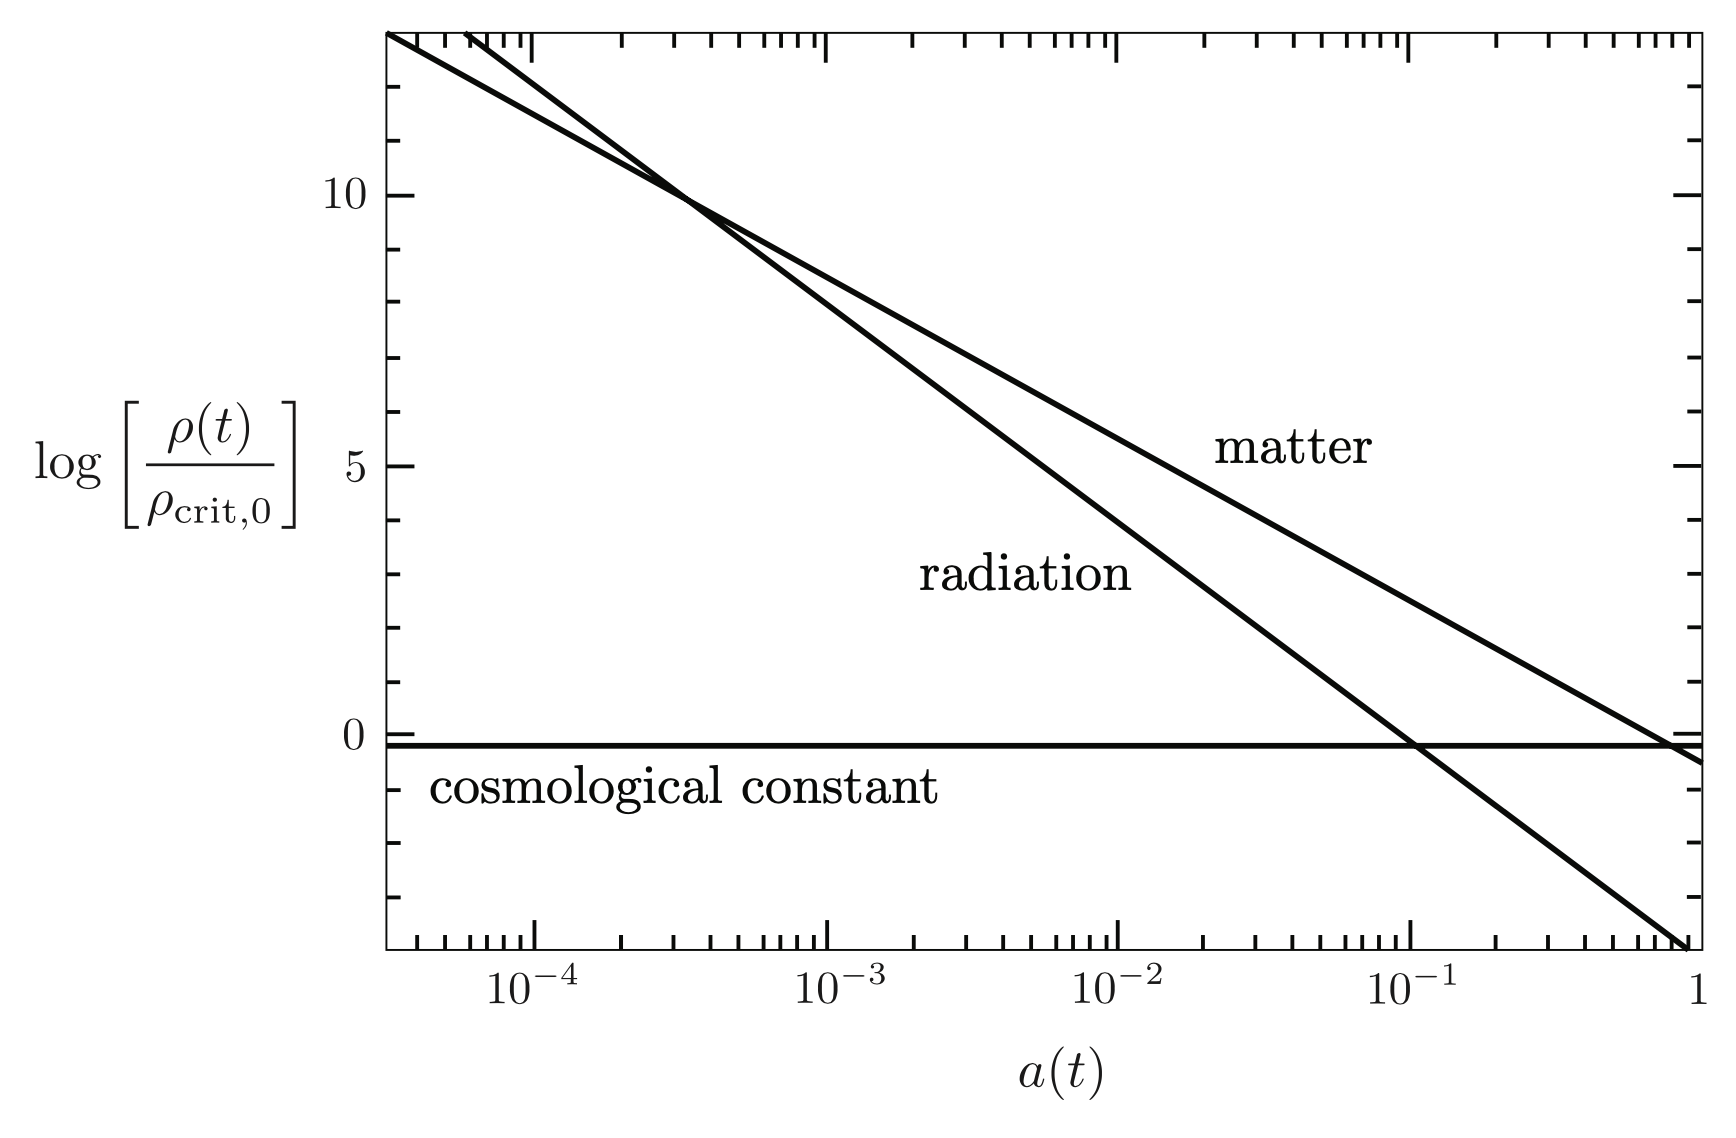
\includegraphics[width=0.95\textwidth]{figures/darkmatter/cosmology.png}
    \caption{Evolution of the energy densities in the universe. Figure reproduced from Ref.~\cite{Baumann2018}.}
    \label{fig:darkmatter:cosmology:energydensity}
\end{figure}


\section{Dark matter relic density}
\label{sec:dm:production}
The early universe was sufficiently hot and dense for dark matter \(\chi\) and other particle species \(f\) to be in thermal equilibrium. Reactions \(\chi \overline{\chi} \leftrightarrow f \overline{f}\) took place with the interaction rate
\begin{align}
    \Gamma = n \langle \sigma v \rangle,
\end{align}
where \(n\) denotes the particle number density and \(\langle\sigma v\rangle\) denotes the thermally averaged product of the interaction cross-section and the average velocity of the particles.
The expansion of the universe decreases the particle number density, until at some point it drops to a point at which interactions hardly occur and dark matter decouples from other particles. The point, at which the interaction rate \(\Gamma|_{T_{\text{dec}}}\) drops below the Hubble expansion \(H|_{T_{\text{dec}}}\), is defined by the decoupling temperature \(T_{\text{dec}}\). This process is referred to \emph{freeze-out} because the dark matter particle number density approaches a constant value for \(T < T_{\text{dec}}\). This constant value is the dark matter relic density.

The dark matter relic density can be derived by solving the Boltzmann equation
\begin{align}
    \frac{\dd{n}}{\dd{t}} = \langle \sigma_{\text{ann}} v \rangle (n_{\text{eq}}^2 - n^2)- 3 H n,
    \label{eq:dm:production:boltzmann}
\end{align}
where \(n_{\text{eq}}\) denotes the particle number density in equilibrium, \(H\) denotes the Hubble constant and \(\langle \sigma_{\text{ann}} v \rangle\) denotes the thermally averaged product of the annihilation cross-section and the velocity of the annihilating particles.

The Boltzmann equation is solved numerically under the condition of constant entropy. The dark matter relic density density in terms of the density parameter and the reduced Hubble constant \(h = H_{0} / \SI{100}{\kilo\meter\per\second\per\mega\parsec} \approx 0.7\) can be approximated as
\begin{align}
    \Omega_{X} h^2 \approx \frac{\SI{3e-27}{\cubic\centi\meter\per\second}}{\langle \sigma_{\text{ann}} v \rangle}.
\end{align}
The dark matter relic density is determined by the annihilation cross-section at the time of the freeze-out.
\Cref{fig:darkmatter:relicabundance:relicabundance} shows the dark matter particle number density as a function of the dimensionless parameter \(x = m_{\chi} / T\). The dotted line corresponds to the evolution of the number density for dark matter remaining in equilibrium without occurrence of any freeze-out. The number density decreases exponentially as a function of \(x\) until the interaction rate becomes too small for dark matter particles to remain in thermal equilibrium, resulting in a constant number density \(N_{X}^{\infty}\) determined by the point of freeze-out \(x_{F} = m_{\chi} / T_{\text{dec}}\). The strength of the interaction defines the dark matter relic density: a large dark matter annihilation cross-section corresponds to a smaller relic density.

\begin{figure}[htbp]
    \centering
    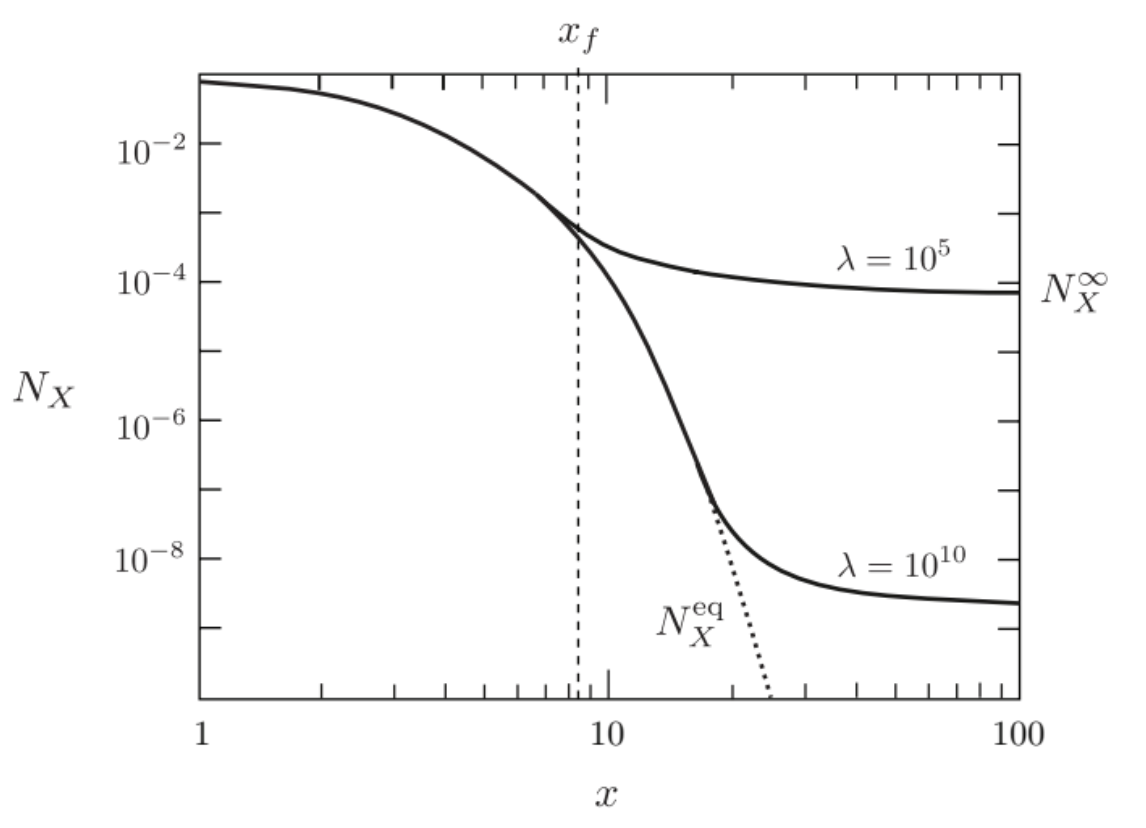
\includegraphics[width=0.9\textwidth]{figures/darkmatter/relicdensity.png}
    \caption{Abundance of dark matter particles \(N_{X}\) in dependence of the dimensionless parameter \(x = m_{\chi} / T\). The freeze-out occurs at the point, where the temperature \(T\) drops below the dark matter particle mass \(m_{\chi}\). The annihilation cross-section is expressed as \(\lambda = \frac{2 \pi^2}{45} g^{\star} \frac{m_{\chi} \langle \sigma_{\text{ann}} v \rangle}{H(m_{\chi})}\), where \(g_{S\star}\) denotes the effective number of degrees of freedom in entropy. Figure reproduced from Ref.~\cite{Baumann2018}.}
    \label{fig:darkmatter:relicabundance:relicabundance}
\end{figure}

For typical weak interaction cross-sections of the order \(\mathcal{O}(\sigma) = \SI{1}{\pico\barn}\) and for a dark matter particle with its mass at the electroweak scale, the observed dark matter relic density \(\Omega_{\chi} h^2 = 0.1188\) is obtained. This striking coincidence is known as the ``WIMP miracle'', referring to the dark matter particle candidate being a weakly interacting massive particle (WIMP).

The simplified calculation discussed here neglects several aspects, which can lead to significant changes in the relic density. It has been shown that the presence of a scalar field in the early universe could modify the value of the relic density. If the dark matter particle mass is similar to other particles, which share a quantum number with the dark matter particle, or if there are several different dark matter particles, co-annihilations occur. In this case, the first term in \Cref{eq:dm:production:boltzmann} needs to account for interactions among the different species, typically resulting in a much more efficient annihilation of dark matter. Radiative corrections in resonant Sommerfeld enhancement are another effect, which can cause dramatic changes in the relic density.


\section{Evidence for dark matter}
\label{sec:dm:evidence}
There is compelling evidence for the existence of dark matter on all astrophysical scales, including rotation curves of gas and stars in galaxies, large samples of galaxy clusters, strong and weak gravitational lensing, distant supernovae, studies of the cosmic microwave background, and large structure formation.

\subsection{Galactic scale}
\label{sec:dm:evidence:galaxy}
The first evidence for the existence of dark matter on sub-galactic scales comes from observations of the Dutch astronomer Jan Oort in 1932. He studied the motion of the stars in our galactic neighbourhood and measured the velocity of stars near the galactic plane by studying their Doppler shifts. His observations found them moving faster than expected --- even so fast that they should be able to escape the gravitational pull of the luminous mass in the Milky Way. Consequentially, he postulated that there must be more galactic mass present to keep the stars on their Keplerian orbits.

The strongest evidence for dark matter on galactic scales is based on the observation of the rotation curves of galaxies. These rotation curves are graphs of the circular velocities of the galaxy's constituents (stars and gas) as a function of their distance from the galactic centre.
\Cref{fig:darkmatter-rotationcurve} shows the rotation curve of the NGC 6503 galaxy.
\begin{figure}[htbp]
    \centering
    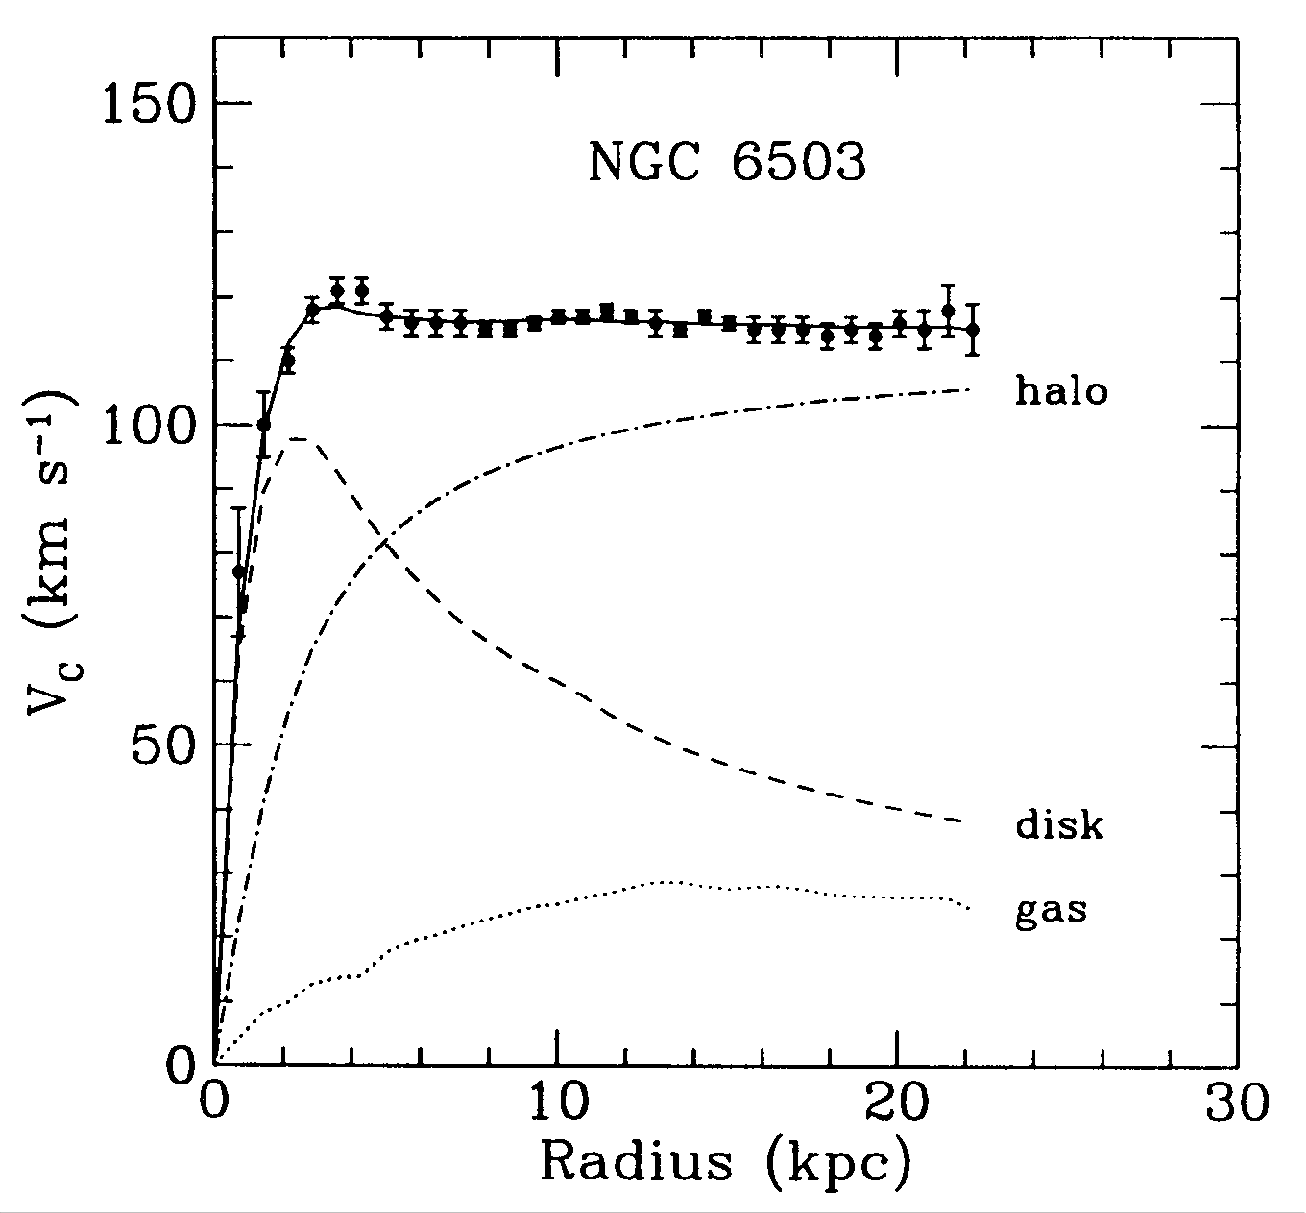
\includegraphics[width=0.95\textwidth]{figures/darkmatter/rotationcurve.png}
    \caption{Galactic rotation curve for NGC 6503 (observed data taken from Ref.~\cite{Burbidge1964}). The decomposition of the rotation curve in contributions from disk and gas potentials shows that an additional contribution due to the dark matter halo is required to match the data. Figure reproduced from Ref.~\cite{Freese2008}.}
    \label{fig:darkmatter-rotationcurve}
\end{figure}
The most striking feature is that the rotation curve approaches a flat shape at large distances, even beyond the edge of the visible disk. The circular velocity of an object on a stable Keplerian orbit is expected to be
\begin{align}
    v(r) = \sqrt{\frac{G M(r)}{r}} = \sqrt{4 \pi G \frac{\int \rho(r) r^2 \dd{r}}{r}},
\end{align}
where \(\rho(r)\) is the mass density profile. Beyond the edge of the visible disk, the rotation curve should be falling proportional to \(1 / \sqrt{r}\). The observation of an approximately constant distribution for large distances implies the existence of a dark matter halo with a mass density profile approaching \(\rho = 1 / r^2\) for large distances. The dark matter halo is expected to fall off faster at some point to keep the total mass of the galaxy finite.

Although there is consensus about the shape of dark matter haloes in the large-distance-limit, the predicted shape in the innermost region of the halo is subject of contention. Cosmological N-body simulations predict dark matter halos with density increasing steeply at small distances (``cusps''). The observed rotation curves of most dwarf galaxies, however, suggest flat, central dark matter density profiles (``cores''). This ``cusp-core problem'' is subject of ongoing investigation.

The velocity dispersion of dwarf spheroidal galaxies (dSphs), small satellite galaxies mostly within \SI{300}{\kilo\parsec} of the Milky Way, is another hint for the existence of dark matter~\cite{Strigari2018}. Dwarf spheroidal galaxies are the nearest, smallest and least luminous galaxies observed to date. They are among the galaxies most strongly dominated by dark matter~\cite{Walker2013}.

Further evidence on galactic scales comes from weak gravitational lensing of distant galaxies by foreground structures~\cite{Bartelmann2016}. Light originating from a luminous source is deflected by a large amount of matter between the source and the observer. The resulting image distortion is known as gravitational lensing and enables the determination of the mass of the foreground structure. Weak gravitational lensing data can provide constraints on the extent and shapes of the galactic dark matter halos~\cite{Hoekstra2002} and gives strong constraints on alternative theories of gravity.


\subsection{Galaxy cluster scale}
\label{sec:dm:evidence:cluster}
The investigation of the velocity dispersion of galaxies in the Coma cluster by Fritz Zwicky arguably pioneered the field of dark matter. Zwicky studied the Doppler-shift of several galaxies in a data set published by Edwin Hubble and Milton Humason and noticed at least eight galaxies with an apparent velocity exceeding \SI{6000}{\kilo\meter\per\second}. For these galaxies to be gravitationally bound, the galaxy cluster is required to have a sufficiently large gravitational potential. Using the virial theorem, he inferred the mass density of the Coma cluster. The estimate for the total mass of the cluster is
\begin{align}
    m_{\text{cluster}} = \sum_{i} m_{\text{galaxy}, i} \approx \frac{2 \langle v^2 \rangle}{G \langle 1 / r\rangle},
\end{align}
where \(\langle v^2 \rangle\) is the average velocity of galaxies in the cluster and \(\langle 1 / r \rangle\) is the average inverse distance between galaxies. Another way to estimate the total mass of the cluster is to measure its luminosity. Comparing the two estimates, he found the estimate based on the cluster's gravitational potential to be 400 times larger than that derived from observations of luminous matter.
Zwicky's use of the phrase ``dunkle (kalte) Materie'' is typically regarded as the first use of the term ``dark matter'' and established the convention of including the photograph of Fritz Zwicky making a silly face in public talks on dark matter.

Zwicky also pioneered the idea that entire galaxy clusters could act as gravitational lenses~\cite{Zwicky1937}. Weak gravitational lensing provides accurate estimates of the total mass of galaxy clusters and thereby provides evidence for the existence of dark matter.
In strong gravitational lensing~\cite{Bartelmann2010}, the light-bending effect is even strong enough to produce multiple images or arcs of the source. If the source, the observer and the matter in between (also called the ``lens'') are aligned, the source is observed in the form of an Einstein ring~\cite{Einstein1936}. The ring's angular radius \(\theta_{E}\) allows estimating the mass \(M\) of the lens via
\begin{align}
    \theta_{E} = \sqrt{4 G M \frac{d_{LS}}{d_{L} d_{S}}},
\end{align}
where \(G\) denotes Newton's constant, \(d_{L}\) denotes the distance to the lens, \(d_{LS}\) denotes the distance between source and lens and \(d_{S}\) denotes the distance to the source.

\Cref{fig:dm:evidence:cluster:abell2218} shows an image of the Abell 2218 galaxy cluster, an exceptionally rich lensing cluster at redshift \(z=0.175\). The galaxies lying behind the cluster's core are magnified and distorted into long arcs, some of them are even multiply imaged. The mass estimated from gravitational lensing exceeds the X-ray based estimate by at least a factor of 2.5~\cite{AbdelSalam1998}.
\begin{figure}[htbp]
    \centering
    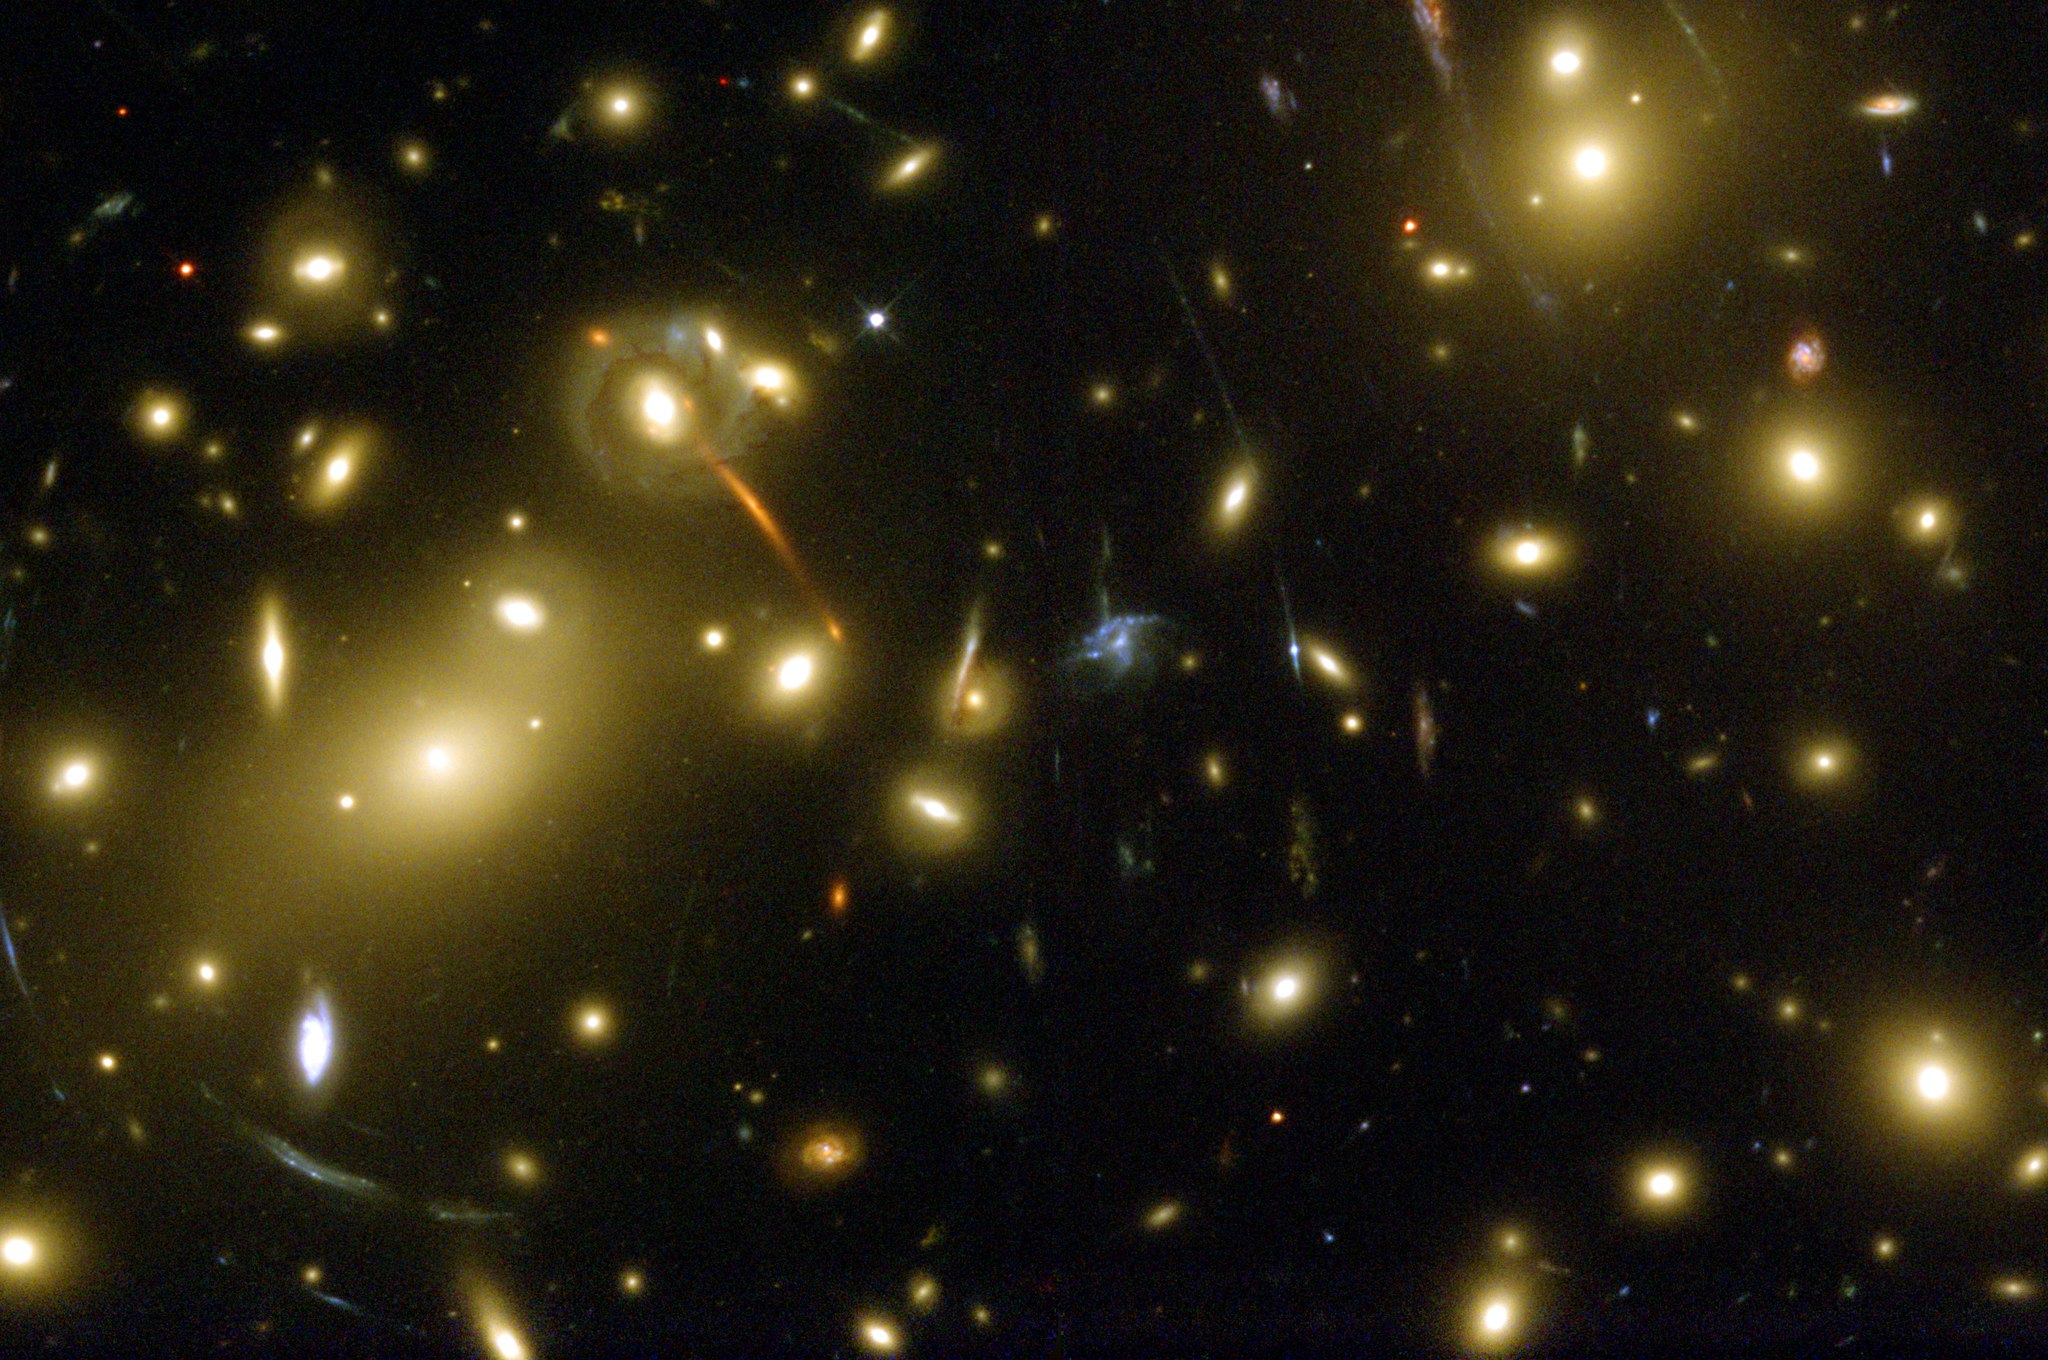
\includegraphics[width=0.95\textwidth]{figures/darkmatter/abell_NGC2218.jpg}
    \caption{Image of the galaxy cluster Abell 2218 and its gravitational lenses, taken by the Hubble space telescope in 1999. Image by Andrew Fruchter (STScI) et al., WFPC2, HST, NASA / Public domain.}
    \label{fig:dm:evidence:cluster:abell2218}
\end{figure}

Arguably the most dramatic evidence for dark matter is provided by observations of the galaxy cluster 1E\num{0657}-\num{558}~\cite{Tucker1998}, also known as ``bullet cluster''. It consists of two sub-clusters of galaxies, which are thought to have previously collided. \Cref{fig:dm:evidence:cluster:bullet} shows images of the bullet cluster from different sources, overlaid with the reconstructed cluster surface mass density \(\kappa\) obtained from weak gravitational lensing. The visible matter of the bullet cluster consists of clouds of hot gas (visible in the optical image), which constitute the majority of the cluster's baryonic matter, and stellar objects (visible in the X-ray image).

The stars are cleanly separated into two distinct sub-clusters, as the probability of individual galaxies colliding is small. In contrast, the clouds of hot gas have interacted ferociously, as the collision of the sub-clusters slowed the gas and left it displaced from the stars. Most of the matter of the sub-clusters, however, is dark matter, which is indicated by the distribution of the reconstructed cluster surface mass density \(\kappa\).

The dark matter in each of the two sub-clusters passed through, seemingly unaffected by the collision. These observations indicate that dark matter interacts weakly both with baryonic matter and with itself. The spatial offset of the centre of the total mass distribution from the centre of the baryonic mass distribution is highly significant (\(8\sigma\)) and gives strong constraints on alternative models of gravity.

\begin{figure}[htbp]
    \centering
    \begin{subfigure}{1.\textwidth}
      \centering
      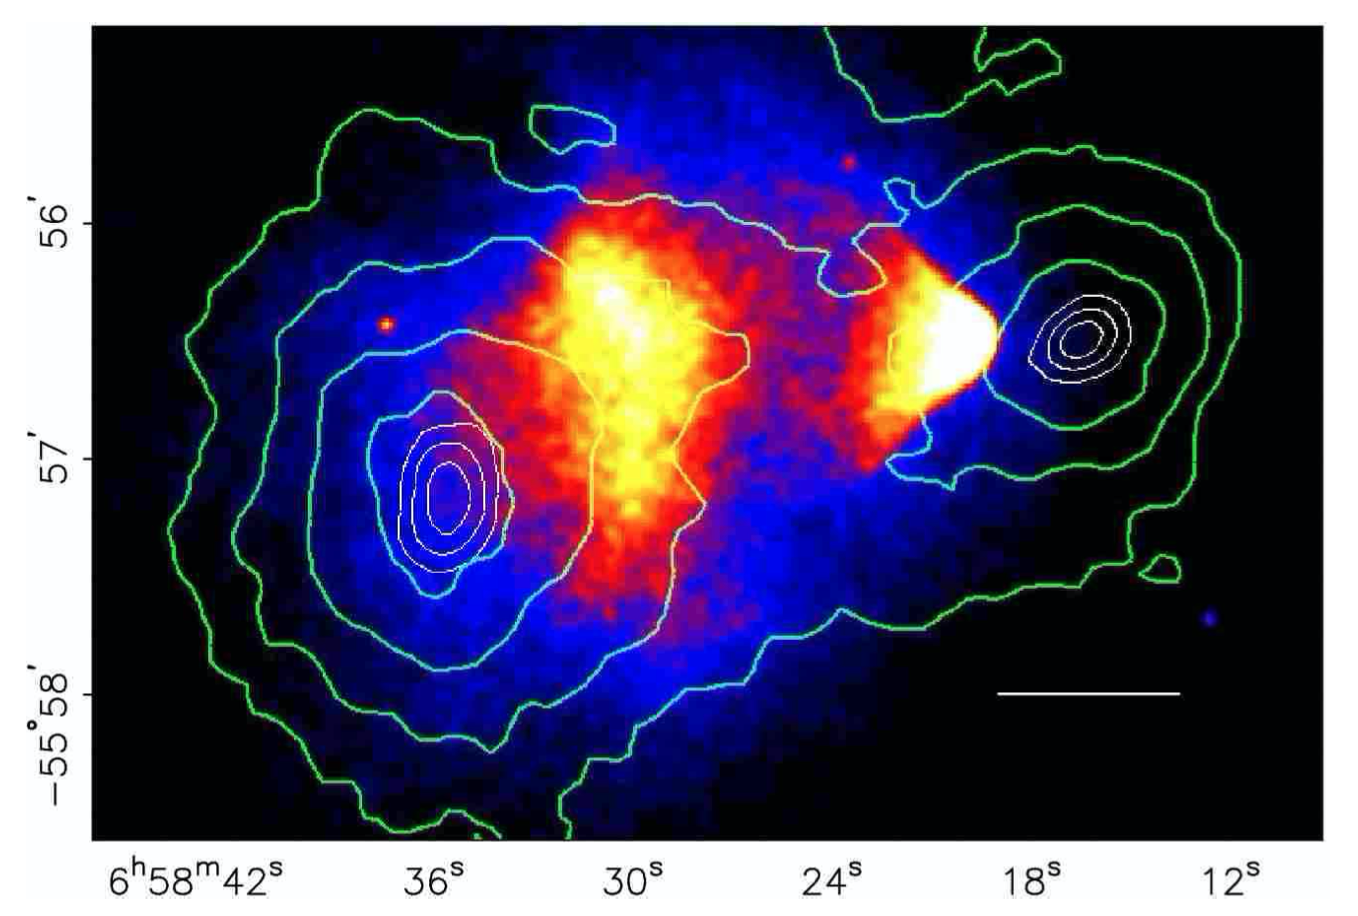
\includegraphics[width=0.95\textwidth]{figures/darkmatter/bulletcluster_magellan.png}
      \caption{Colour image of 1E\num{0657}-\num{558} from the \SI{6.5}{\meter} Magellan telescopes located at the Las Campanas observatory, Chile.}
      \label{fig:dm:evidence:cluster:bullet:magellan}
    \end{subfigure}
    \\
    \begin{subfigure}{1.\textwidth}
      \centering
      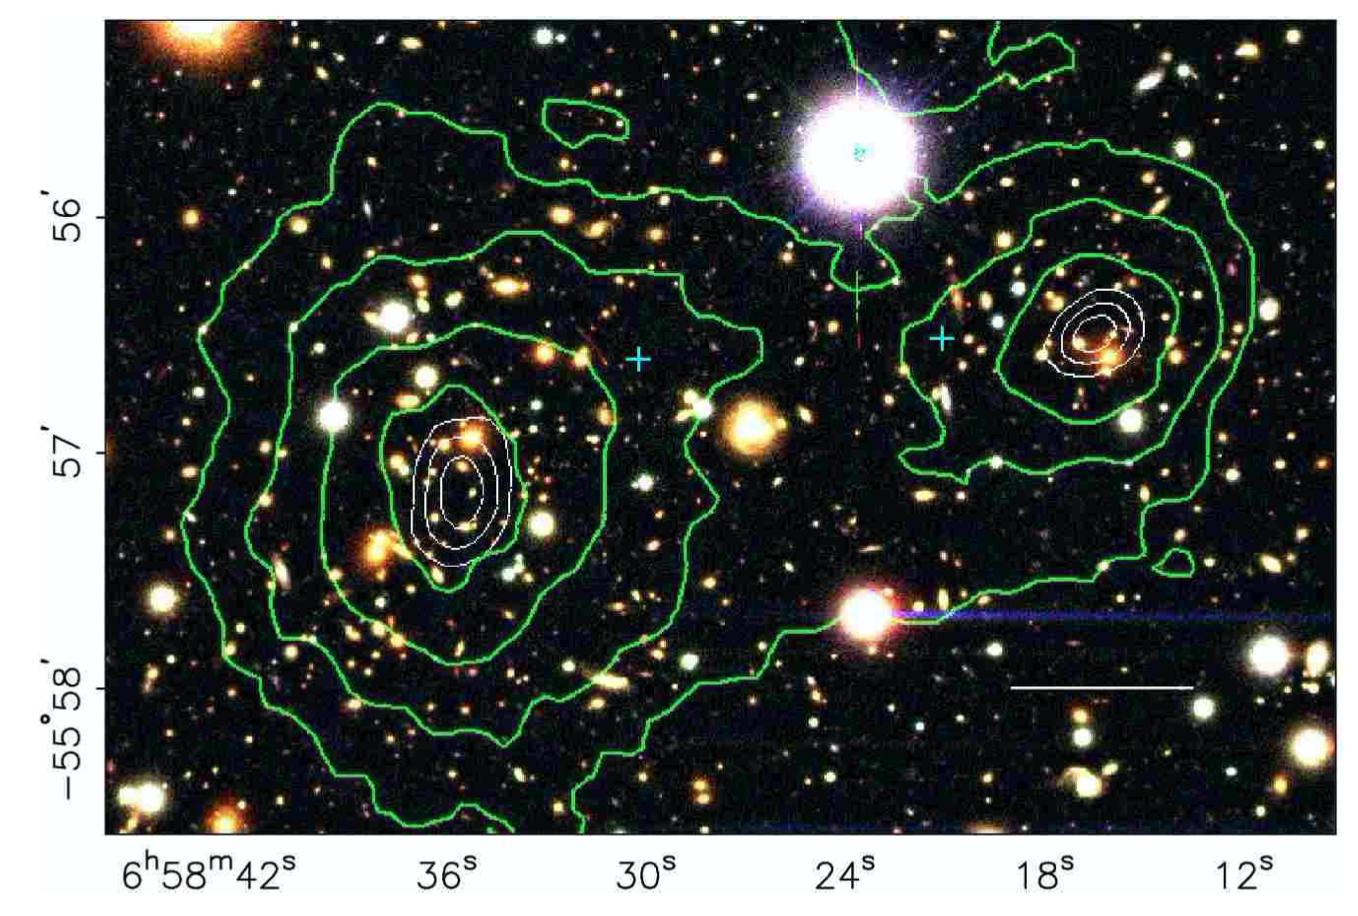
\includegraphics[width=.95\textwidth]{figures/darkmatter/bulletcluster_chandra.png}
      \caption{X-ray image of 1E\num{0657}-\num{558} from NASA Chandra satellite observatory.}
      \label{fig:dm:evidence:cluster:bullet:chandra}
    \end{subfigure}
    \caption{Images of 1E\num{0657}-\num{558} based on optical (top) and X-ray observations (bottom). The green contours of the reconstructed cluster surface mass density \(\kappa\) obtained from weak gravitational lensing are overlaid in both images. The three white contours show the uncertainty in the position of the two primary galaxy concentration centres, corresponding to \(1\sigma\), \(2\sigma\), and \(3\sigma\) confidence levels. Figures reproduced from Ref.~\cite{Clowe2006}.}
    \label{fig:dm:evidence:cluster:bullet}
\end{figure}


\subsection{Cosmological scale}
\label{sec:dm:evidence:cosmology}
Although the evidence on the scales of galaxies and galaxy clusters for themselves is compelling, the observations do not allow for an estimate of the total amount of dark matter in the universe. This information can be extracted from the analysis of cosmic microwave background data.

The cosmic microwave background (CMB), which was discovered in 1965 by Arno Penzias and Robert Wilson~\cite{Penzias1965}, is electromagnetic radiation with a black body radiation spectrum at temperature \(T_{\text{CMB}} = \SI{2.72548 \pm 0.00057}{\kelvin}\)~\cite{Fixsen2009}. It consists of primordial photons created in the early universe, which were in thermal equilibrium (c.f. the discussion for dark matter particles in \Cref{sec:dm:production}). Photons and free electrons frequently interacted via scattering processes, as space was filled by a charged plasma. The interaction rate decreased when the electrons combined with protons to form electrically neutral hydrogen atoms. Consequentially, the photons decoupled and could propagate undisturbed. The CMB can be thought of as the sphere of the last scattering with the observer in the centre and allows probing the conditions in the early universe directly.

In the last three decades, the CMB has been mapped by experiments with increasing precision~\cite{Smoot1992,Bennett2003,Spergel2003,Spergel2007,Reichardt2009,Planck2019,Planck2020}. The almost uniform temperature of the CMB suggests a phase of rapid, inflationary expansion of the universe, which is driven by the cosmological constant \(\Lambda\).
After subtracting the dipole moment associated with the movement of the earth, the CMB exhibits temperature fluctuations with the characteristic scale \(\delta T / T_{\text{CMB}} \approx 10^{-5}\). These tiny fluctuations are used to determine the cosmological parameters. The temperature fluctuations are parametrised as an expansion in spherical harmonics \(Y_{lm}(\theta, \varphi)\)\footnote{The base mode \(l=0\) corresponds to the CMB temperature \(T_{\text{CMB}}\). The first mode \(l=1\) corresponds to the dipole anisotropy. Therefore, the expansion in the fluctuations starts at \(l=2\).}
\begin{align}
    \frac{\delta T}{T_{\text{CMB}}} (\theta, \varphi) &= \sum_{l=2}^{\infty} \sum_{m=-l}^{l} a_{lm} Y_{lm}(\theta, \varphi).
\end{align}

Assuming the values of the coefficients \(a_{lm}\) are independent of the index \(m\), it is possible to define the observed angular power spectrum
\begin{align}
    C^{TT}_{l} = \frac{1}{2l+1} \sum_{m=-l}^{l} \abs{a_{lm}}^2
\end{align}
for discrete values of the multi-pole moment \(l \propto \pi / \phi\). The CMB map and the power spectrum measured by PLANCK~\cite{Planck2019} is shown in \Cref{fig:dm:evidence:cosmology:cmb}.

\begin{figure}[htbp]
    \centering
    \begin{subfigure}{1.\textwidth}
      \centering
      \includegraphics[width=0.95\textwidth]{figures/darkmatter/cmb_planck_map.png}
      \caption{CMB sky map. The grey line delineates a region, which lies mostly around the Galactic plane, where residuals from foreground emission are expected to be substantial and which is therefore masked in the analysis.}
      \label{fig:dm:evidence:cosmology:cmb:map}
    \end{subfigure}
    \\
    \begin{subfigure}{1.\textwidth}
      \centering
      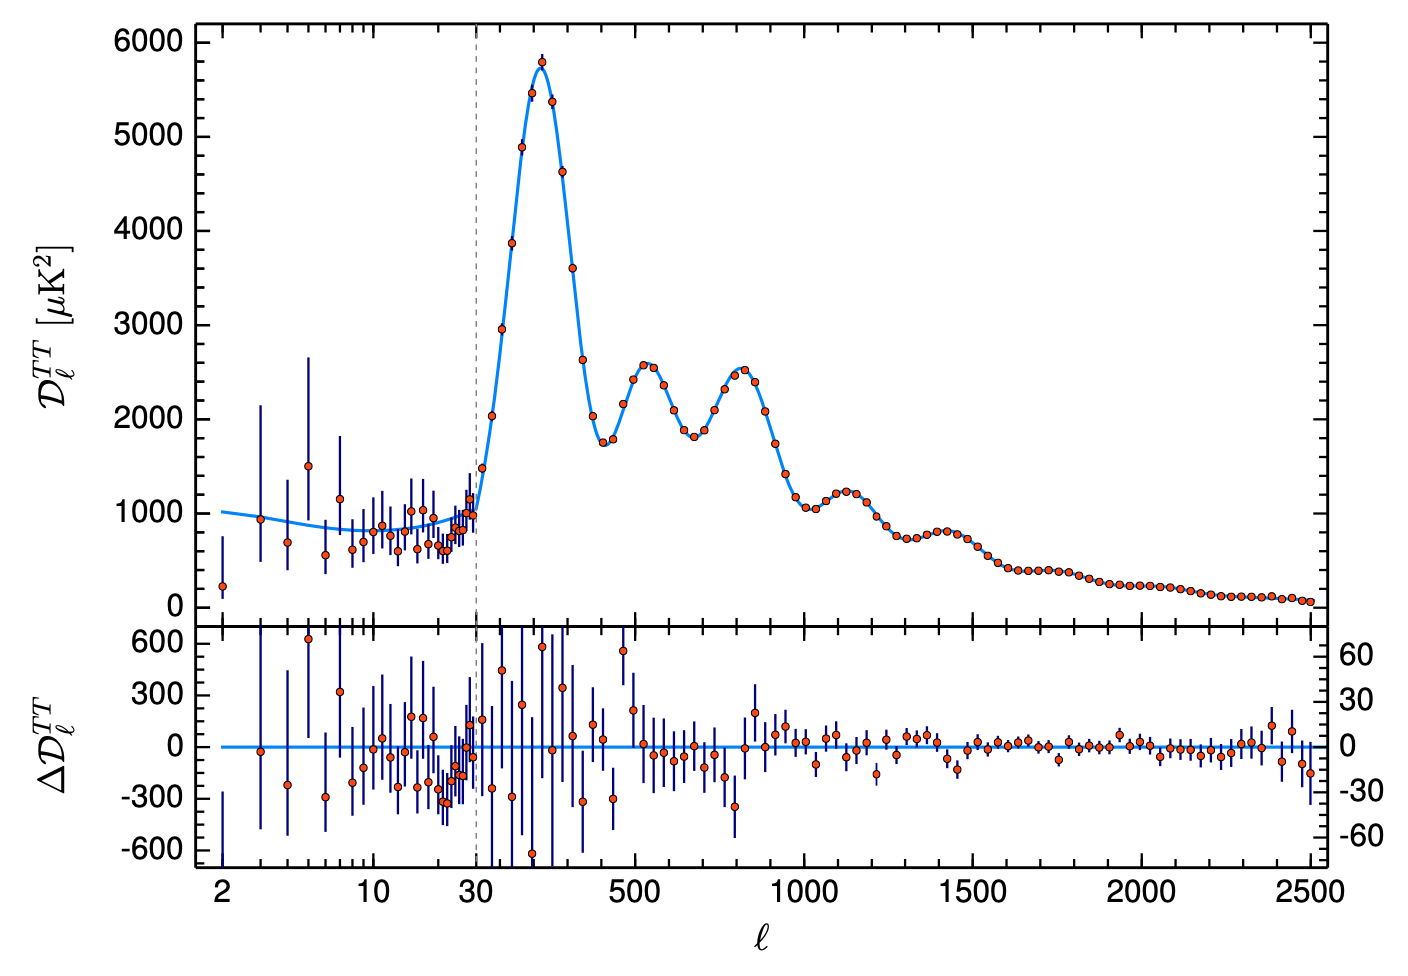
\includegraphics[width=.95\textwidth]{figures/darkmatter/cmb_planck_spectrum.png}
      \caption{CMB temperature power spectrum. The upper panel shows the scaled power spectrum modes \(D^{TT}_{l}= l(l+1) C^{TT}_{l} / (2\pi) \). The \(\Lambda\)-CDM model best fit to the data is overlaid in light blue in the upper panel. The residuals with respect to this model are shown in the lower panel. For better visualisation, the horizontal scale changes at \(l=30\) from a logarithmic scale to a linear scale.}
      \label{fig:dm:evidence:cosmology:cmb:spectrum}
    \end{subfigure}
    \caption{Planck (2018) observations of the CMB. Figures reproduced from Refs.~\cite{Planck2019} (top) and \cite{Planck2020} (bottom).}
    \label{fig:dm:evidence:cosmology:cmb}
\end{figure}

The measured power spectrum consists of a set of peaks, which each define an angular scale with particularly large contributions to the temperature fluctuations. The cosmological parameters can be inferred from a fit of the positions, shapes and relative sizes of the peaks in the spectrum. The peaks originate from acoustic waves in the baryon-photon fluid before the photon decoupling. These acoustic waves can be understood as the competing effects of gravity and radiative pressure. The baryon-photon fluid gets pulled into gravitational wells around regions of considerable matter accumulation. As more baryonic matter accumulates, the increasing photon pressure acts against the gravitational potential of the wells.

Even-numbered peaks are associated with the compression of the baryon-photon fluid due to gravity, whereas odd-numbered peaks are associated with the counteracting effect of radiative pressure. A higher baryon content in the baryon-photon fluid corresponds to smaller radiative pressure and larger compression peaks. Therefore, the relative amplitude between odd- and even-numbered peaks is a measure of the baryon density parameter \(\Omega_{b}\). Dark matter only contributes to the gravitational wells and does not respond to radiative pressure. The size of the third peak indicates a sizeable dark matter component at the time of the last scattering. The first peak corresponds to waves, which have only compressed once. Its position is used to determine the spatial curvature parameter \(\kappa\).

The estimates for the products of the cosmological density parameters and reduced Hubble constant \(h\)~\cite{Planck2020} are
\begin{itemize}
    \item baryon density parameter \(\Omega_{b} h^2 = \num{0.02237} \pm \num{0.00015}\)
    \item dark matter (DM) density parameter \(\Omega_{\text{DM}} h^2 = \num{0.1200} \pm \num{0.0012}\).
\end{itemize}
The estimates are compatible with the predictions from Big Bang nucleosynthesis~\cite{Simha2008} and with those obtained from the Sloan Digital Sky Survey~\cite{Tegmark2004}.

A global fit of the \(\Lambda\)-CDM model allows constraining the amount of dark energy by extracting the
\begin{itemize}
    \item cosmological constant density parameter \(\Omega_{\Lambda} = \num{0.6847} \pm \num{0.0073}\).
\end{itemize}
The knowledge of these fundamental cosmological parameters allows for a breakdown of the present composition of the universe in \SI{4.9}{\percent} baryonic matter, \SI{26.8}{\percent} dark matter and \SI{68.3}{\percent} dark energy.

The current structure of the universe is a result of the initial matter fluctuations in the early universe.
The temperature fluctuations in the CMB indicate that the early universe was not entirely homogeneous and isotropic. These density fluctuations have grown into the galaxies and galaxy clusters observed today. However, this could not have been achieved by baryonic matter alone.

Structure formation could only have occurred after the universe cooled down sufficiently for the photons to decouple. Then, however, there would not have been sufficient time to form the amount of structure observed today. Dark matter, on the other hand, is thought to decouple from the photons much earlier. Its density perturbations can form the gravitational wells acting as a seed for the gravitational collapse of visible matter. The observed large scale structure of the universe is compatible with the cold dark matter hypothesis~\cite{Blumenthal1984}.


\section{Candidates for dark matter particles}
\label{sec:dm:candidates}
It would be an understatement to say that several compelling candidates for dark matter have been proposed. The parameter space of dark matter models is vast and covers at least \num{30} orders of magnitude in the mass and \num{40} orders of magnitude in the interaction cross-section with protons~\cite{Ibarra2015}.

In analogy to the example of hidden planets in the Solar System in \Cref{sec:dm:intro}, one could naively assume dark matter to consist of yet unobserved baryonic matter.
Massive Astrophysical Compact Halo Objects (MACHOs)~\cite{Griest1993}, compact objects much less luminous but otherwise equivalent to ordinary stars, were among the first dark matter candidates. Possibilities for such objects include planets, brown dwarfs, neutron stars, Jupiter-like objects, and black holes. However, searches based on micro-lensing surveys and determinations of the cosmic baryon density from measurements of the primordial light element abundances and the CMB data strongly constrain the fraction of the dark matter constituted by MACHOs~\cite{Bertone2018}.

There are several compelling candidates for a non-baryonic dark matter particle. A suitable dark matter particle candidate must be able to be probed experimentally and needs to satisfy the following conditions~\cite{Taoso2008}:
\begin{enumerate}
    \item It has to be an electrically neutral,~\cite{McDermott2011} stable~\cite{Audren2014} particle with sufficiently low interactions to match the appropriate relic density~\cite{Srednicki1988}.
    \item It must lead to sufficiently low velocity during decoupling to allow for the observed large scale structure formation in the universe.
    \item It has to be compatible with the constraints
    \begin{itemize}
        \item on its self-interactions~\cite{Randall2008,Tulin2018},
        \item due to stellar evolution~\cite{Scott2009},
        \item from Big Bang nucleosynthesis~\cite{Kawasaki2015}
        \item from direct searches for dark matter~\cite{Liu2017},
        \item from indirect searches for dark matter~\cite{Conrad2017},
        \item from collider searches for dark matter~\cite{Buchmueller2017}, and
        \item due to other astrophysical observations.
    \end{itemize}
\end{enumerate}

A possible non-baryonic dark matter candidate in the SM appears to be the neutrino, as it has the ``undisputed virtue of being known to exist''~\cite{Bergstroem2000}. Neutrinos are neutral, have non-vanishing mass and only interact weakly with SM particles. They are an example of hot dark matter since they are still relativistic at the time of their decoupling due to their small mass \(m_{\nu} < \SI{1}{\electronvolt}\)~\cite{Aker2019}. However, neutrinos alone are not able to account for the total dark matter mass in the universe. The relic density parameter for neutrinos with mass \(\sum_{i} m_{\nu_{i}} = \SI{0.264}{\electronvolt}\) is predicted to be~\cite{Loureiro2019}
\begin{align}
    \Omega_{\nu} h^2 \approx \sum_{i} \frac{m_{\nu_{i}}}{\SI{92.5}{\electronvolt}} \lesssim 0.00285.
\end{align}
The relic density parameter is too small for neutrinos to be the dominant component of dark matter. Furthermore, the observed amount of structure in galaxy clustering is inconsistent with the predictions for a neutrino-dominated universe~\cite{White1984}.

These arguments prove that the SM does not contain a viable candidate for a dark matter particle. However, several extensions of the SM predict viable candidates:

\textbf{Sterile neutrinos}~\cite{Dodelson1994,Boyarsky2019} are right-handed (\(\text{SU}(2)_{L}\) singlet) neutrinos, which do not interact with SM particles except by small mixing \(\theta\) with left-handed \(\text{SU}(2)_{L}\)-active neutrinos. They can overcome the constraints which ruled out the SM neutrinos as dark matter. The mass of sterile neutrinos is expected to be in the \si{\kilo\electronvolt}-range. Although sterile neutrinos are expected to decay predominantly to three left-handed neutrinos, their radioactive decay mode to one left-handed neutrino and a photon gives rise to a quasi-monochromatic photon line at half the sterile neutrino-mass and can be exploited for searches.
%An overview of current constraints on thermally produced sterile neutrinos is shown in \Cref{fig:dm:candidates:constraints:sterile-neutrinos}.

\textbf{Axions} are very light pseudo-scalar bosons, which have been originally proposed as a solution to preserve \(CP\) symmetry in strong interactions~\cite{Peccei1977}. Axion-like-particles (ALPs) define a more general class of very light, weakly coupled  bosons, which are excellent candidates for particle dark matter in the ALP mass range \(\SI{e-6}{\electronvolt} < m_{A} < \SI{e-2}{\electronvolt}\)~\cite{Graham2015}. The main search strategy for axion searches is based on the axion-photon conversion in external magnetic fields.
%An overview of current constraints on axions is shown in \Cref{fig:dm:candidates:constraints:axions}.

% \begin{figure}[htbp]
%     \centering
%     \begin{subfigure}{.95\textwidth}
%       \centering
%       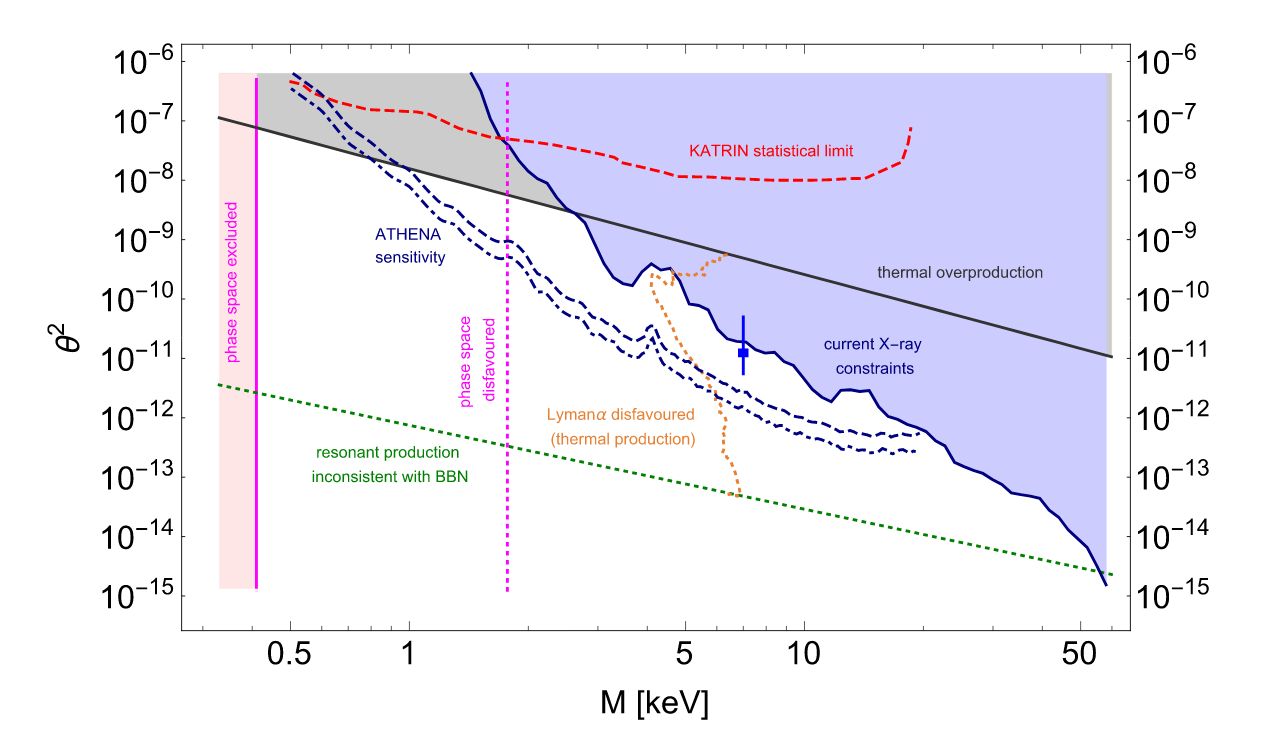
\includegraphics[width=1.\textwidth]{figures/darkmatter/sterile_neutrino.png}
%       \caption{Constraints on thermally produced sterile neutrinos in the plane defined by the sterile neutrino mass and the mixing \(\theta\) with SM neutrinos. The solid lines indicate largely model-independent constraints from phase-space considerations for fermionic dark matter in dSphs (pink), from current non-observations of X-rays from the decay of sterile neutrinos to photons and SM neutrinos (violet), and from the observed relic density (black). Further constraints originate from Big Bang nucleosynthesis (green) and structure formation (orange). The expected sensitivity improvements from the ATHENA X-ray telescope~\cite{Neronov2016} data is overlaid. Also, the expected sensitivity of the TRISTAN upgrade of the KATRIN experiment~\cite{Mertens2019} is indicated (red).}
%       \label{fig:dm:candidates:constraints:sterile-neutrinos}
%     \end{subfigure}
%     \\
%     \begin{subfigure}{1.\textwidth}
%       \centering
%       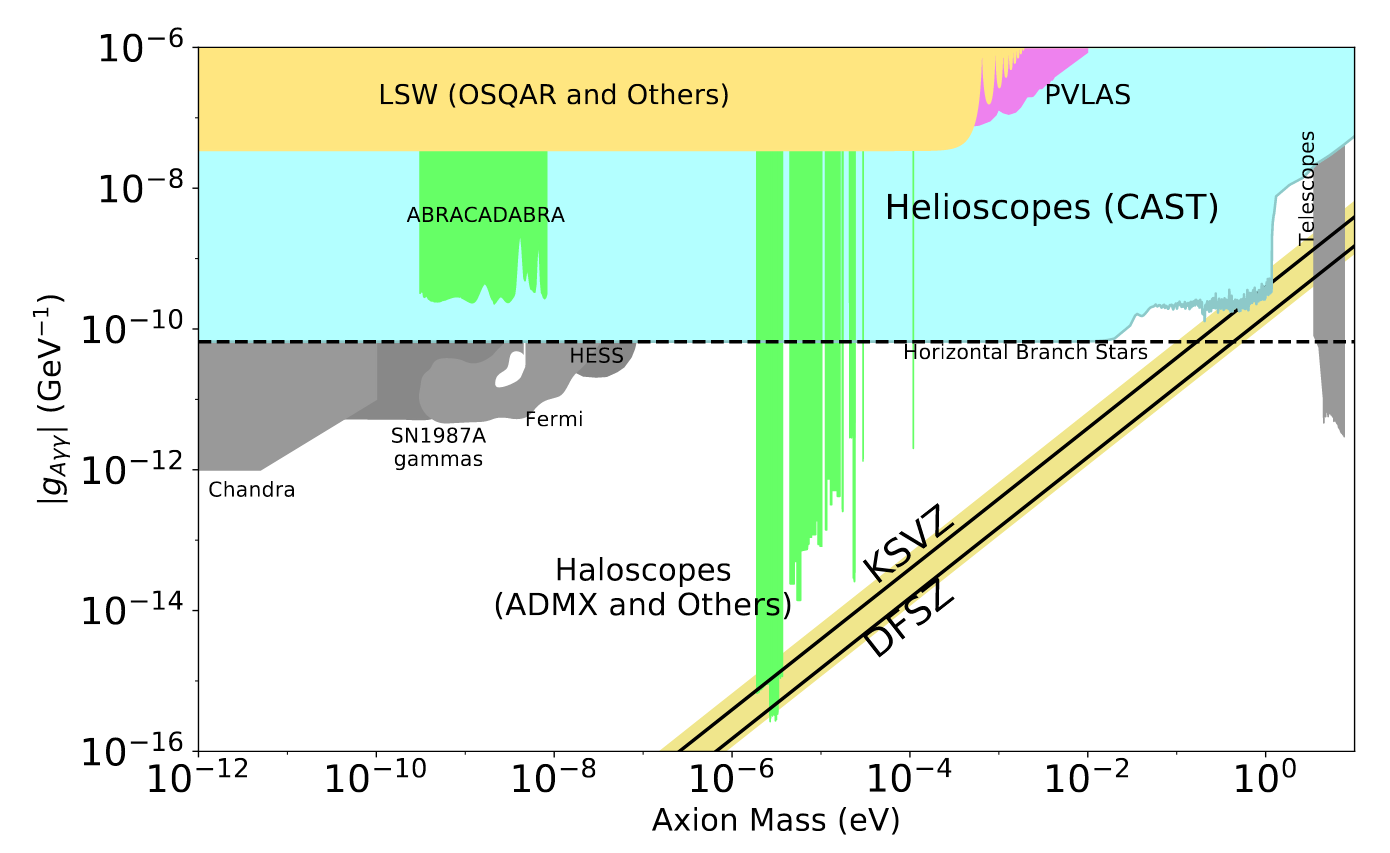
\includegraphics[width=.9\textwidth]{figures/darkmatter/axions.png}
%       \caption{Constraints on axions in the plane defined by the axion mass and the axion to two-photon coupling strength \(g_{A\gamma\gamma}\). The upper orange region is excluded by light-shining-through-wall (LSW) experiments, the purple region is excluded by searches for vacuum magnetic birefringence (PVLAS), the green regions are excluded by direct searches using haloscopes, the upper blue region is excluded by helioscope experiments searching for solar axions, and the light and dark grey regions are excluded by astrophysical observations. The diagonal yellow band indicates predictions of typical QCD axion models (KSVZ, DSFZ).}
%       \label{fig:dm:candidates:constraints:axions}
%     \end{subfigure}
%     \caption{Constraints on selected non-baryonic dark matter candidates. Figures reproduced from Refs.~\cite{Boyarsky2019} (top) and \cite{Tanabashi2018} (bottom).}
%     \label{fig:dm:candidates:constraints}
% \end{figure}

The \textbf{WIMP} paradigm (weakly interacting massive particle, denoted as \(\chi\)) defines a class of particularly well-motivated candidates for dark matter particles. WIMPs are neutral, stable or very long-lived particles. The interactions of WIMPs with the SM occur with similar strength as typical electroweak interactions. The WIMP mass is expected to range from \(\SI{10}{\giga\electronvolt} < m_{\chi} < \SI{100}{\tera\electronvolt}\)~\cite{Kolb1990,Griest1990}. Therefore, thermally produced WIMPs are non-relativistic by the time of decoupling and are a typical example of cold dark matter. Consequentially, the WIMP paradigm provides a simple mechanism to obtain the observed relic density, which is referred to as the ``WIMP miracle'' (c.f. \Cref{sec:dm:production}).
In regions of large WIMP density, they can annihilate and produce a flux of \(\gamma\)-rays, anti-particles and neutrinos. WIMP searches are discussed in detail in \Cref{sec:dm:searches}.

A notable example of a framework predicting WIMPs is the minimal supersymmetric extension of the SM (MSSM)~\cite{Fox2019}. In this model, the lightest supersymmetric particle (LSP), whose decay to SM particles is prohibited by a custodial symmetry, is a WIMP. Other theories predicting WIMPs include theories with extra-dimensions~\cite{Cheng2002} with Kaluza-Klein states, Little Higgs models~\cite{Birkedal2006} with the lightest \(T\)-odd particle, or technicolor theory~\cite{Kainulainen2007} with a massive fourth family neutrino, to name only a few.

The dark matter searches discussed in this dissertation focus on the WIMP paradigm.


\section{Search for WIMP dark matter}
\label{sec:dm:searches}
There are several complementary approaches to search for dark matter:
\begin{itemize}
    \item direct detection experiments measure the recoil of dark matter particles in the vicinity of the Earth on nuclei in the active detector material.
    \item indirect detection experiments search for an excess in the particle flux observed by earth-bound and satellite detectors due to pair annihilation of dark matter particles in regions of enhanced dark matter density.
    \item searches for dark matter at particle colliders investigate signatures of missing momentum in the detector plane transverse to the colliding beams due to dark matter pair production.
\end{itemize}
The experimental approaches for detecting the interactions of dark matter particles with SM particles are complementary. While direct and indirect detection experiments can establish the galactic origin of a signal, their sensitivity to the details of the interaction between dark matter and SM particles is limited. Collider searches, on the other hand, are unable to probe the lifetime of dark matter particles beyond the time scale required for traversing the detector but can probe their interactions in greater detail~\cite{Buchmueller2017}.
\Cref{fig:darkmatter:searches:overview} shows the relevant momentum ranges in the different kinds of searches with prototypical Feynman graphs.
\begin{figure}[htbp]
    \centering
    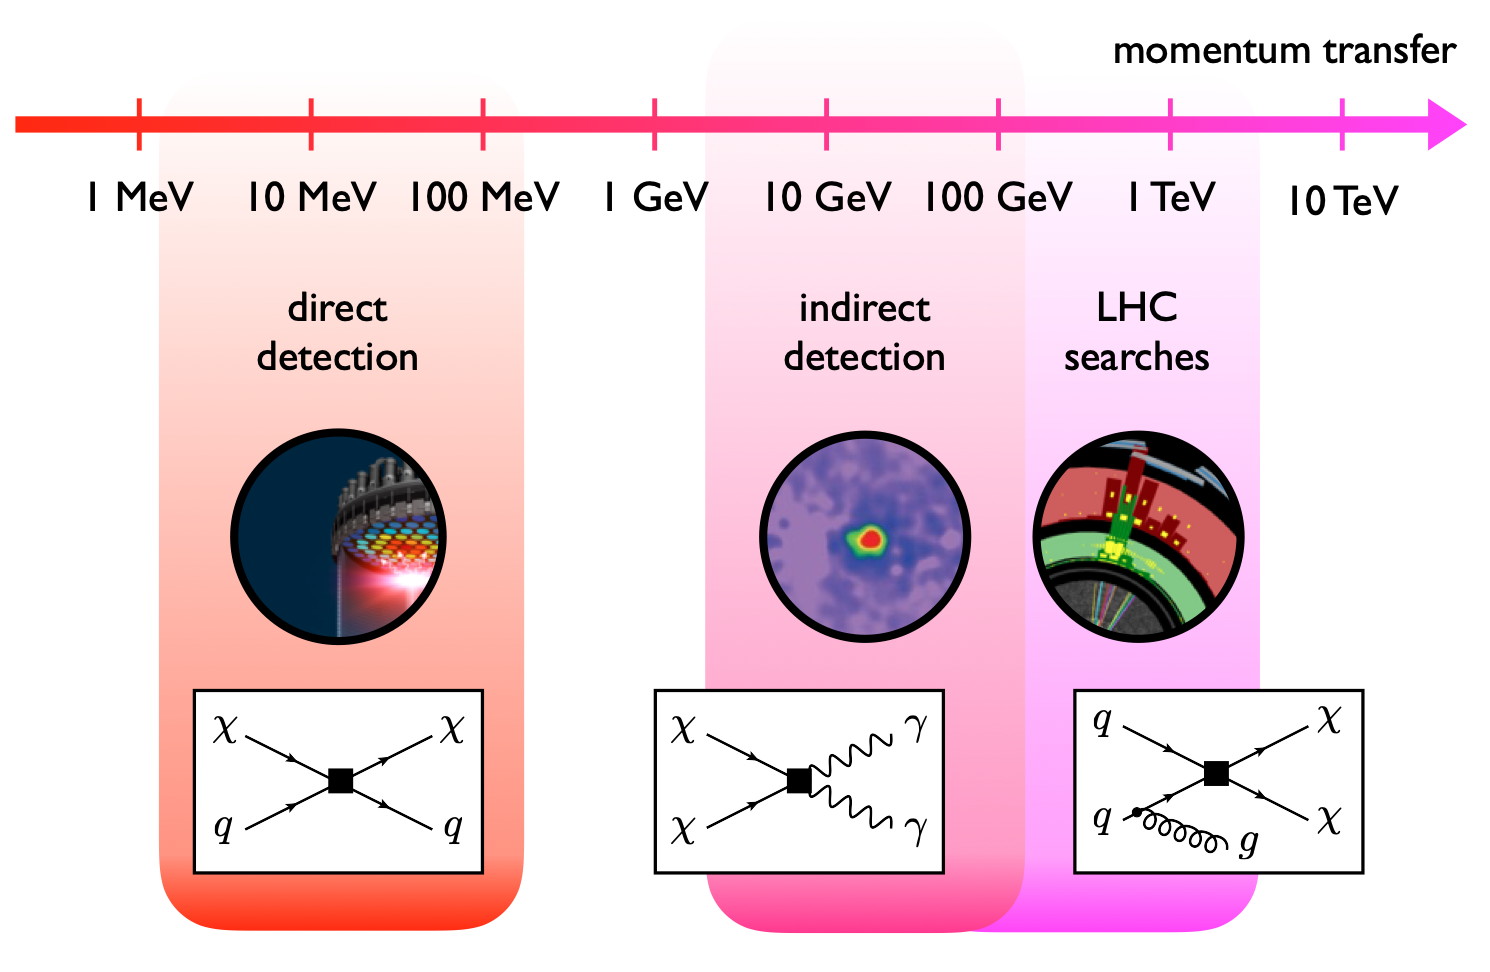
\includegraphics[width=0.9\textwidth]{figures/darkmatter/overview_searches.png}
    \caption{Range of momentum transfers probed by direct detection experiments, indirect detection experiments and collider searches with prototypical Feynman graphs illustrating the underlying processes. Figure reproduced from Ref.~\cite{Abe2020}.}
    \label{fig:darkmatter:searches:overview}
\end{figure}


\subsection{Direct detection experiments}
\label{sec:dm:searches:dd}
Direct detection experiments (c.f. Refs.~\cite{Liu2017,Schumann2019} for a review) aim to detect the nuclear recoil in the scattering of galactic WIMPs off target nuclei. The interaction rate of WIMPs with nuclei in the detector~\cite{Bertone2005}
\begin{align}
    R \approx \sum_{i} N_{i} n_{\chi} \langle \sigma_{i \chi} \rangle
\end{align}
depends on
\begin{itemize}
    \item the number of target nuclei \(N_{i} = m_{\text{detector}} / m_{A_{i}}\) in the active detector material for nucleons of species \(i\) with atomic weight \(A_{i}\),
    \item the local WIMP density \(n_{\chi} = \rho_{\chi} / m_{\chi}\), where \(\rho_{\chi}\) is the local WIMP energy density and \(m_{\chi}\) is the WIMP mass, and
    \item the cross-section \(\sigma_{i \chi}\) for interactions between WIMPs and nucleons of species \(i\), averaged over the relative WIMP velocity with respect to the detector.
\end{itemize}
The values of the astrophysical parameters are set to typical assumptions~\cite{Schumann2019} for the Solar System. The canonical value for the local WIMP energy density is \(\rho_{\chi} = \SI{0.3}{\giga\electronvolt\per\cubic\centi\meter}\). The WIMP velocity distribution \(f(\vec{v})\) is defined by the mean WIMP velocity \(v_{c} \approx \SI{220}{\kilo\meter\per\second}\) at the solar distance from the galactic centre and by the galactic escape velocity \(v_{\text{esc}} \approx \SI{544}{\kilo\meter\per\second}\), which determines the truncation of \(f(\vec{v})\).
The remaining free parameters are the WIMP mass \(m_{\chi}\) and the WIMP-nucleon interaction cross-section. The exclusion limits obtained from the non-observation of WIMP signals are usually shown as contours in the plane defined by these two parameters.

The primary signal in direct detection experiments are nuclear recoils. For WIMPs with mass in the range \(\SI{1}{\giga\electronvolt} < m_{\chi} < \SI{1}{\tera\electronvolt}\), the typical elastic recoil energy of the atomic nucleus ranges from \(\SI{1}{\kilo\electronvolt} < E_{\text{recoil}} < \SI{100}{\kilo\electronvolt}\). Electron recoil events can also be investigated, although their typical recoil energy is smaller.

The nuclear recoil energy can be converted into
\begin{itemize}
    \item thermal motion (phonons),
    \item ionisation (electrons) of the detector material,
    \item scintillation light (photons) through the Coulomb field of the charged nucleus.
\end{itemize}
These modes define the different detection channels of direct detection experiments. Typically, two channels are combined to achieve more powerful discrimination against electron recoil backgrounds from radioactivity.

Direct detection experiments require a very low background environment because of the meagre interaction rates for WIMP-nucleon interactions. Therefore, direct detection experiments are hosted in deep underground laboratories to suppress background produced by cosmic rays. Also, they employ passive shielding and active vetoes to suppress external backgrounds and are made of high-purity detector components to minimise internal backgrounds.
As the experiments increase their sensitivity to lower recoil energies, an irreducible background from the scattering of atmospheric and solar neutrinos becomes an issue. This background is referred to as the ``neutrino floor'' and poses new challenges to the future generation of experiments.

WIMP-nucleon scattering can be classified depending on the type of WIMP-nucleon coupling in
\begin{itemize}
    \item spin-independent (SI) interactions, which are mediated by scalar or vector couplings, with coherent and elastic WIMP scattering off all nucleons in the nucleus, and
    \item spin-dependent (SD) interactions, which are mediated by axial-vector couplings, with a \(J(J+1)\) dependence of the cross-section on the nuclear spin \(J\).
\end{itemize}
SI interactions give a larger signal than SD interactions because of the coherent scattering and the ensuing \(A^2\) dependence of the interaction cross-section on the atomic weight. SD interactions can be studied in WIMP-proton scattering of \ch{^{19}_{9}Fl} and in WIMP-neutron scattering of \ch{^{73}_{32}Ge}, \ch{^{129}_{54}Xe}, and \ch{^{131}_{54}Xe}.

Direct detection experiments can be based on
\begin{itemize}
    \item liquid noble gas detectors, such as Xenon (XENON1T~\cite{Aprile2017}, LUX~\cite{Akerib2013}, PandaX-II~\cite{Tan2016}) or Argon (DEAP-3600~\cite{Amaudruz2018}, DarkSide-50~\cite{Agnes2018}), which are sensitive mostly to small cross-sections,
    \item cryogenic crystals, such as Calcium tungstate (CRESST-III~\cite{Abdelhameed2019}) or Germanium (SuperCDMS~\cite{Agnese2018}, CDMSlite~\cite{Agnese2019}), which are sensitive mostly to small masses,
    \item crystal scintillators, such as Sodium iodide (DAMA/LIBRA~\cite{Bernabei2018}).
\end{itemize}

The DAMA/LIBRA~\cite{Bernabei2018} experiment has reported an annually modulated signal consistent with a WIMP interpretation. However, the results are in conflict with non-observations and resulting exclusion limits obtained from other experiments.
\Cref{fig:dm:searches:dd:si} shows an overview of the constraints placed on the SI WIMP-nucleon cross-section for WIMPs with mass \(m_{\chi}\).
% \Cref{fig:dm:searches:dd:si} and \Cref{fig:dm:searches:dd:sd} show an overview of the constraints placed on the SI and SD WIMP-nucleon cross-sections for WIMPs with mass \(m_{\chi}\), respectively.
\begin{figure}[htbp]
    \centering
    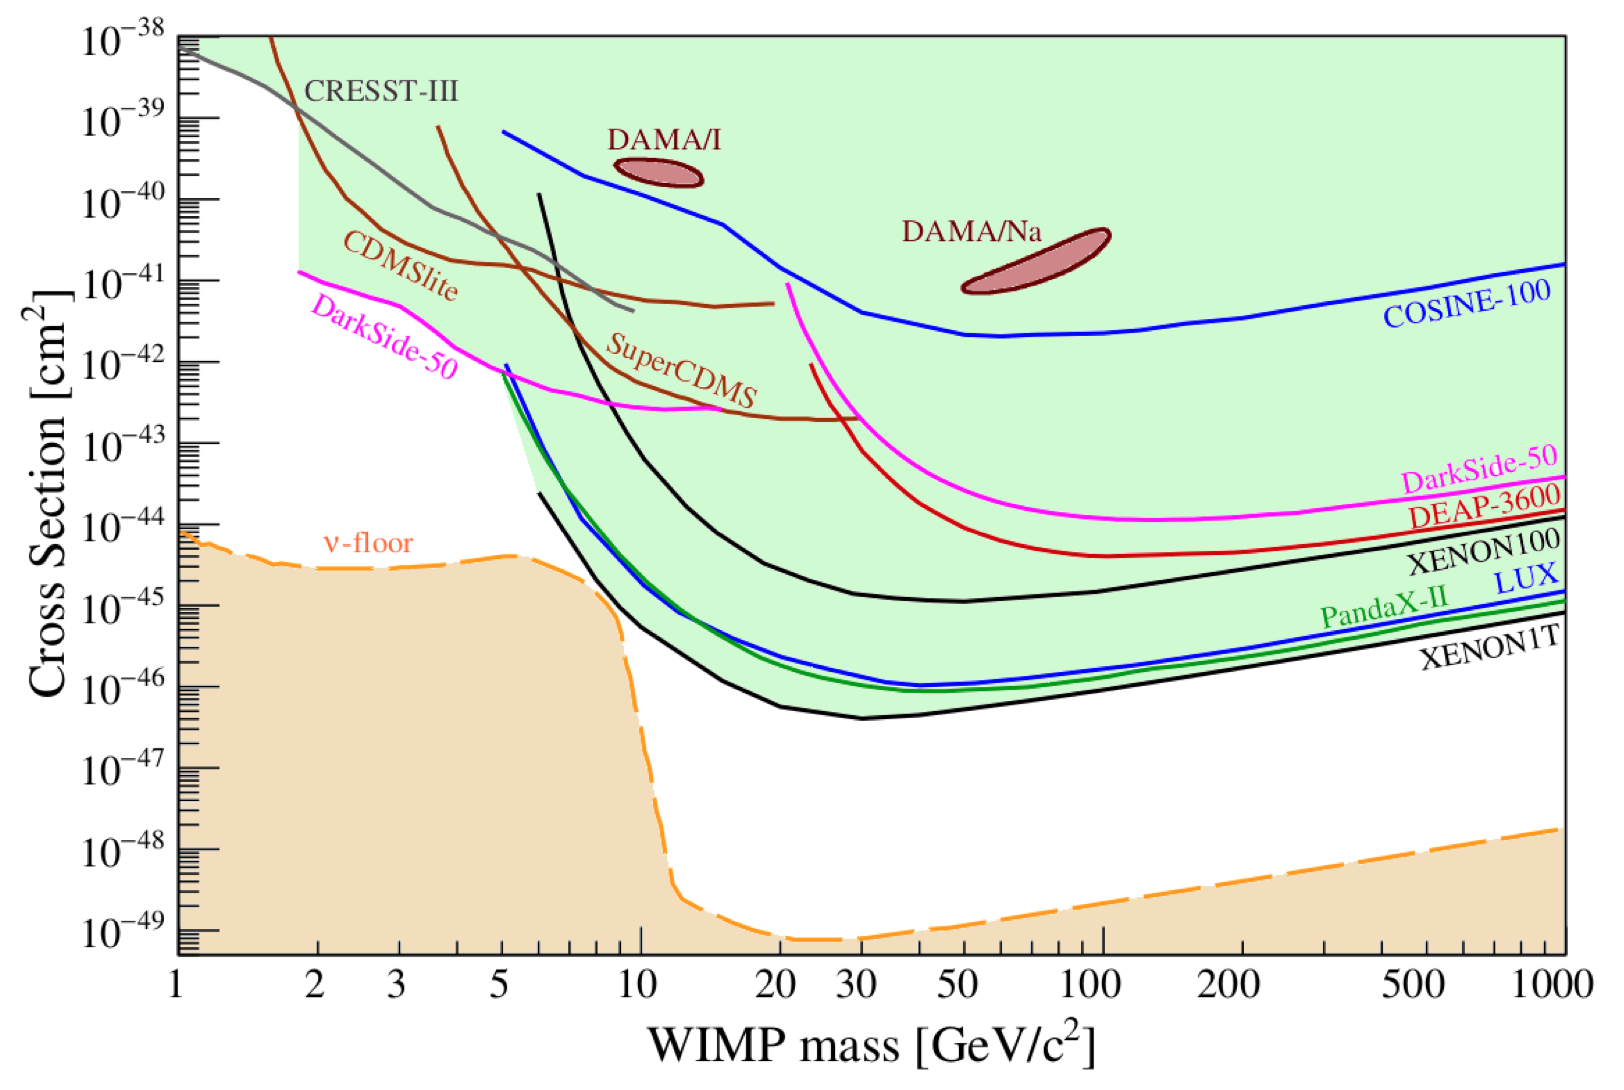
\includegraphics[width=0.95\textwidth]{figures/darkmatter/directdetection2019_si.png}
    \caption{Constraints placed on the SI WIMP-nucleon cross-section for WIMPs with mass \(m_{\chi}\) by direct detection experiments. Figure reproduced from Ref.~\cite{Schumann2019}.}
    \label{fig:dm:searches:dd:si}
\end{figure}

% \begin{figure}[htbp]
%     \centering
%     \begin{subfigure}{1.\textwidth}
%       \centering
%       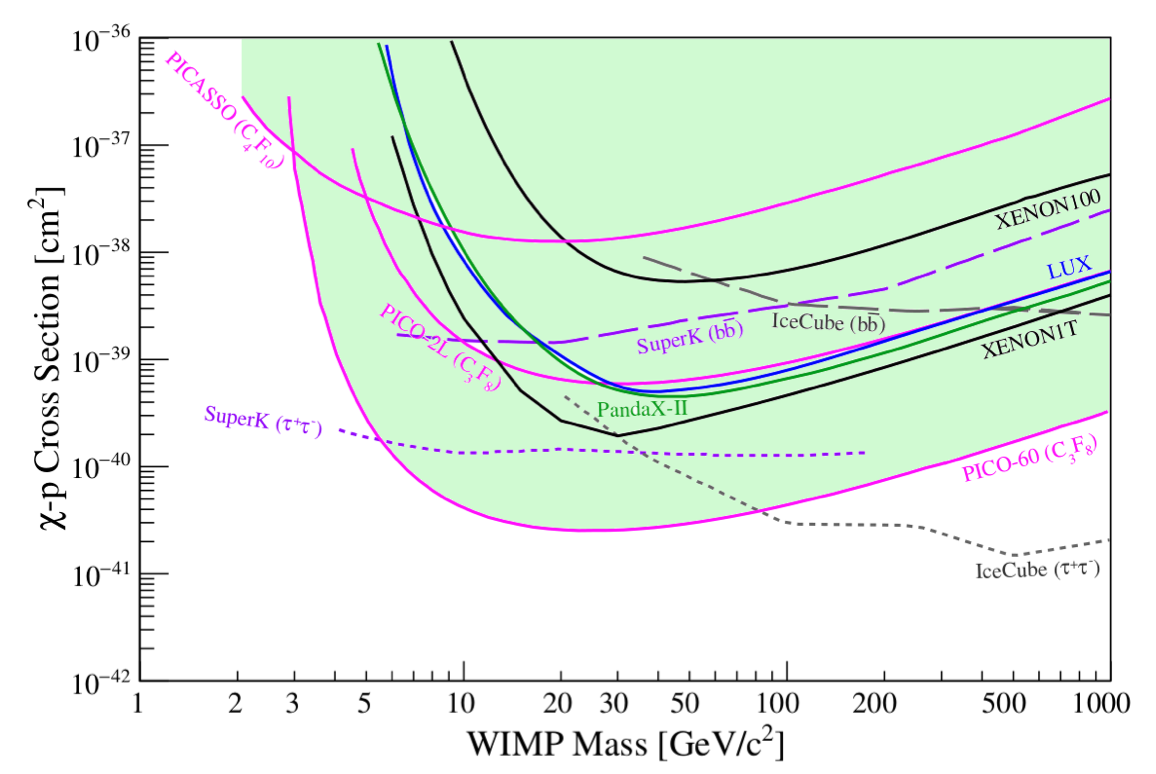
\includegraphics[width=.95\textwidth]{figures/darkmatter/directdetection2019_sdp.png}
%       \caption{WIMP-proton interactions}
%       \label{fig:dm:searches:dd:sd:wimp-proton}
%     \end{subfigure}
%     \\
%     \begin{subfigure}{1.\textwidth}
%       \centering
%       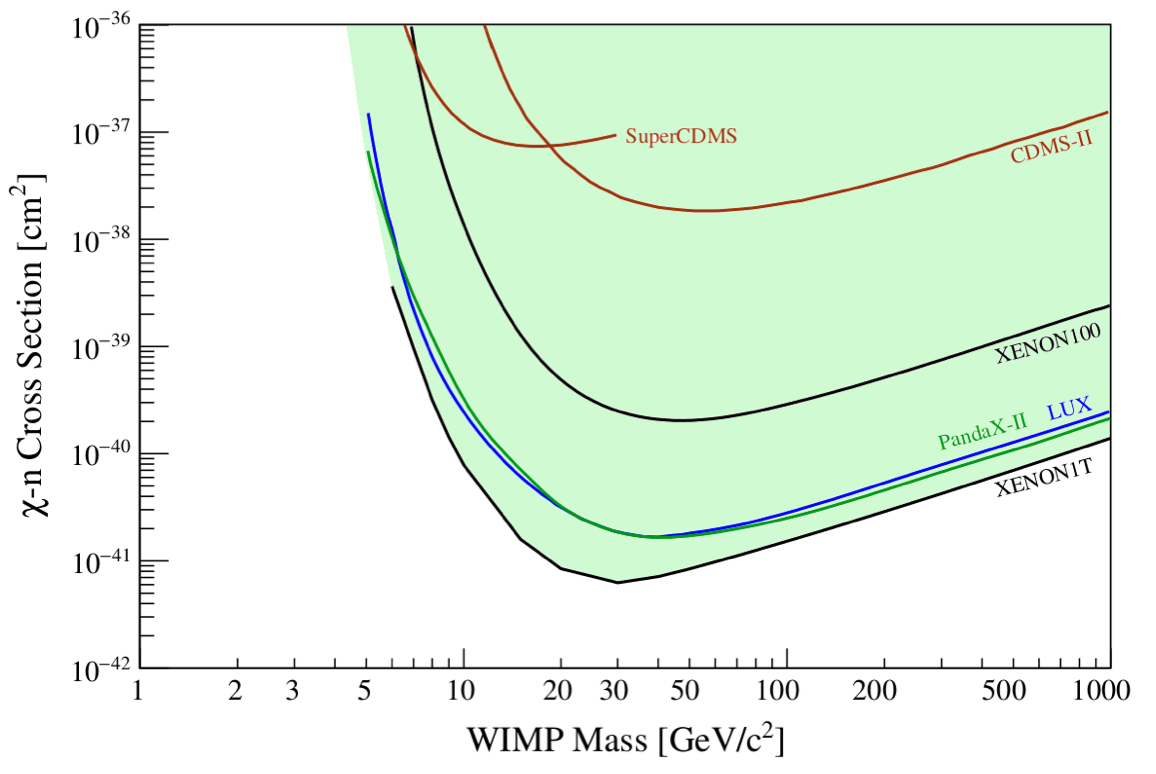
\includegraphics[width=.95\textwidth]{figures/darkmatter/directdetection2019_sdn.png}
%       \caption{WIMP-neutron interactions}
%       \label{fig:dm:candidates:constraints:axions}
%     \end{subfigure}
%     \caption{Constraints placed on the SD WIMP-nucleon cross-section for WIMPs with mass \(m_{\chi}\) by direct detection experiments. Figure reproduced from Ref.~\cite{Schumann2019}.}
%     \label{fig:dm:searches:dd:sd}
% \end{figure}

\subsection{Indirect detection experiments}
\label{sec:dm:searches:id}
Indirect detection experiments (c.f. Refs.~\cite{Conrad2017,losHeros2020} for a review) search for excess in flux of gamma rays, neutrinos or cosmic rays due to dark matter pair annihilation. WIMPs can annihilate in regions of large density, such as galaxy cores, the Sun or the Earth.

The gamma-ray, neutrino or cosmic ray flux (denoted \(x\)) from an object under consideration~\cite{losHeros2020}
\begin{align}
    \frac{\dd{\phi}}{\dd{E}_{x}} = \frac{1}{4 \pi} \frac{\langle \sigma_{\HepProcess{\chi \chi \to X}} v\rangle}{2 m_{\chi}^2} \frac{\dd{N_{x}}}{\dd{E_{x}}} \times \int \dd{\Omega} \int_{\text{line of sight}} \dd{r} \rho_{\chi}(r)^2
\end{align}
depends on
\begin{itemize}
    \item the thermally averaged product of the dark matter self-annihilation cross-section times the dark matter velocity \(\langle \sigma_{\HepProcess{\chi \chi \to X}} v\rangle\)
    \item the WIMP mass \(m_{\chi}\)
    \item the expected particle spectrum \(\dd{N_{x}}\dd{E_{x}}\), and
    \item the so-called ``J-factor'', the integrated squared dark matter density along the line of sight to the object under consideration \(\int_{\text{line of sight}} \rho_{\chi}(r)^2 \dd{r} \dd{\Omega}\).
\end{itemize}

Searches for gamma-ray emission have focused on nearby dwarf spheroidal galaxies with considerably low backgrounds, the inner region of the Milky Way with a considerable background at almost any wavelength, and nearby clusters of galaxies. A potential signal of dark matter annihilation manifests as a nearly mono-energetic line in the spectrum, with an energy close to the WIMP mass and a width proportional to the dark matter velocity~\cite{Tanabashi2018}.

A variety of different experiments aim for indirect detection of dark matter. The Fermi Large Area Telescope (LAT)~\cite{Atwood2009} and the ground-based facilities HESS~\cite{Aharonian2006}, VERITAS~\cite{Archambault2017}, HAWC~\cite{Abeysekara2018}, and MAGIC~\cite{Aleksi2016} probe the gamma-ray spectrum for WIMPs in the mass range \(\SI{1}{\giga\electronvolt} < m_{\chi} < \SI{10}{\tera\electronvolt}\). Fermi LAT observed an excess emission at energies of a few GeV in the gamma-ray flux from the galactic centre. Although several interpretations suggest compatibility with a potential signal~\cite{Hooper2011,Karwin2017}, this interpretation is subject of contestation~\cite{deBoer2017}.
Additional experiments looking for indirect detection are AMS~\cite{Aguilar2013}, PAMELA~\cite{Adriani2009}, and IceCube~\cite{Aartsen2013}.

\Cref{fig:dm:searches:id:overview} shows an overview of constraints on WIMPs from indirect detection experiments.
\begin{figure}[htbp]
    \centering
    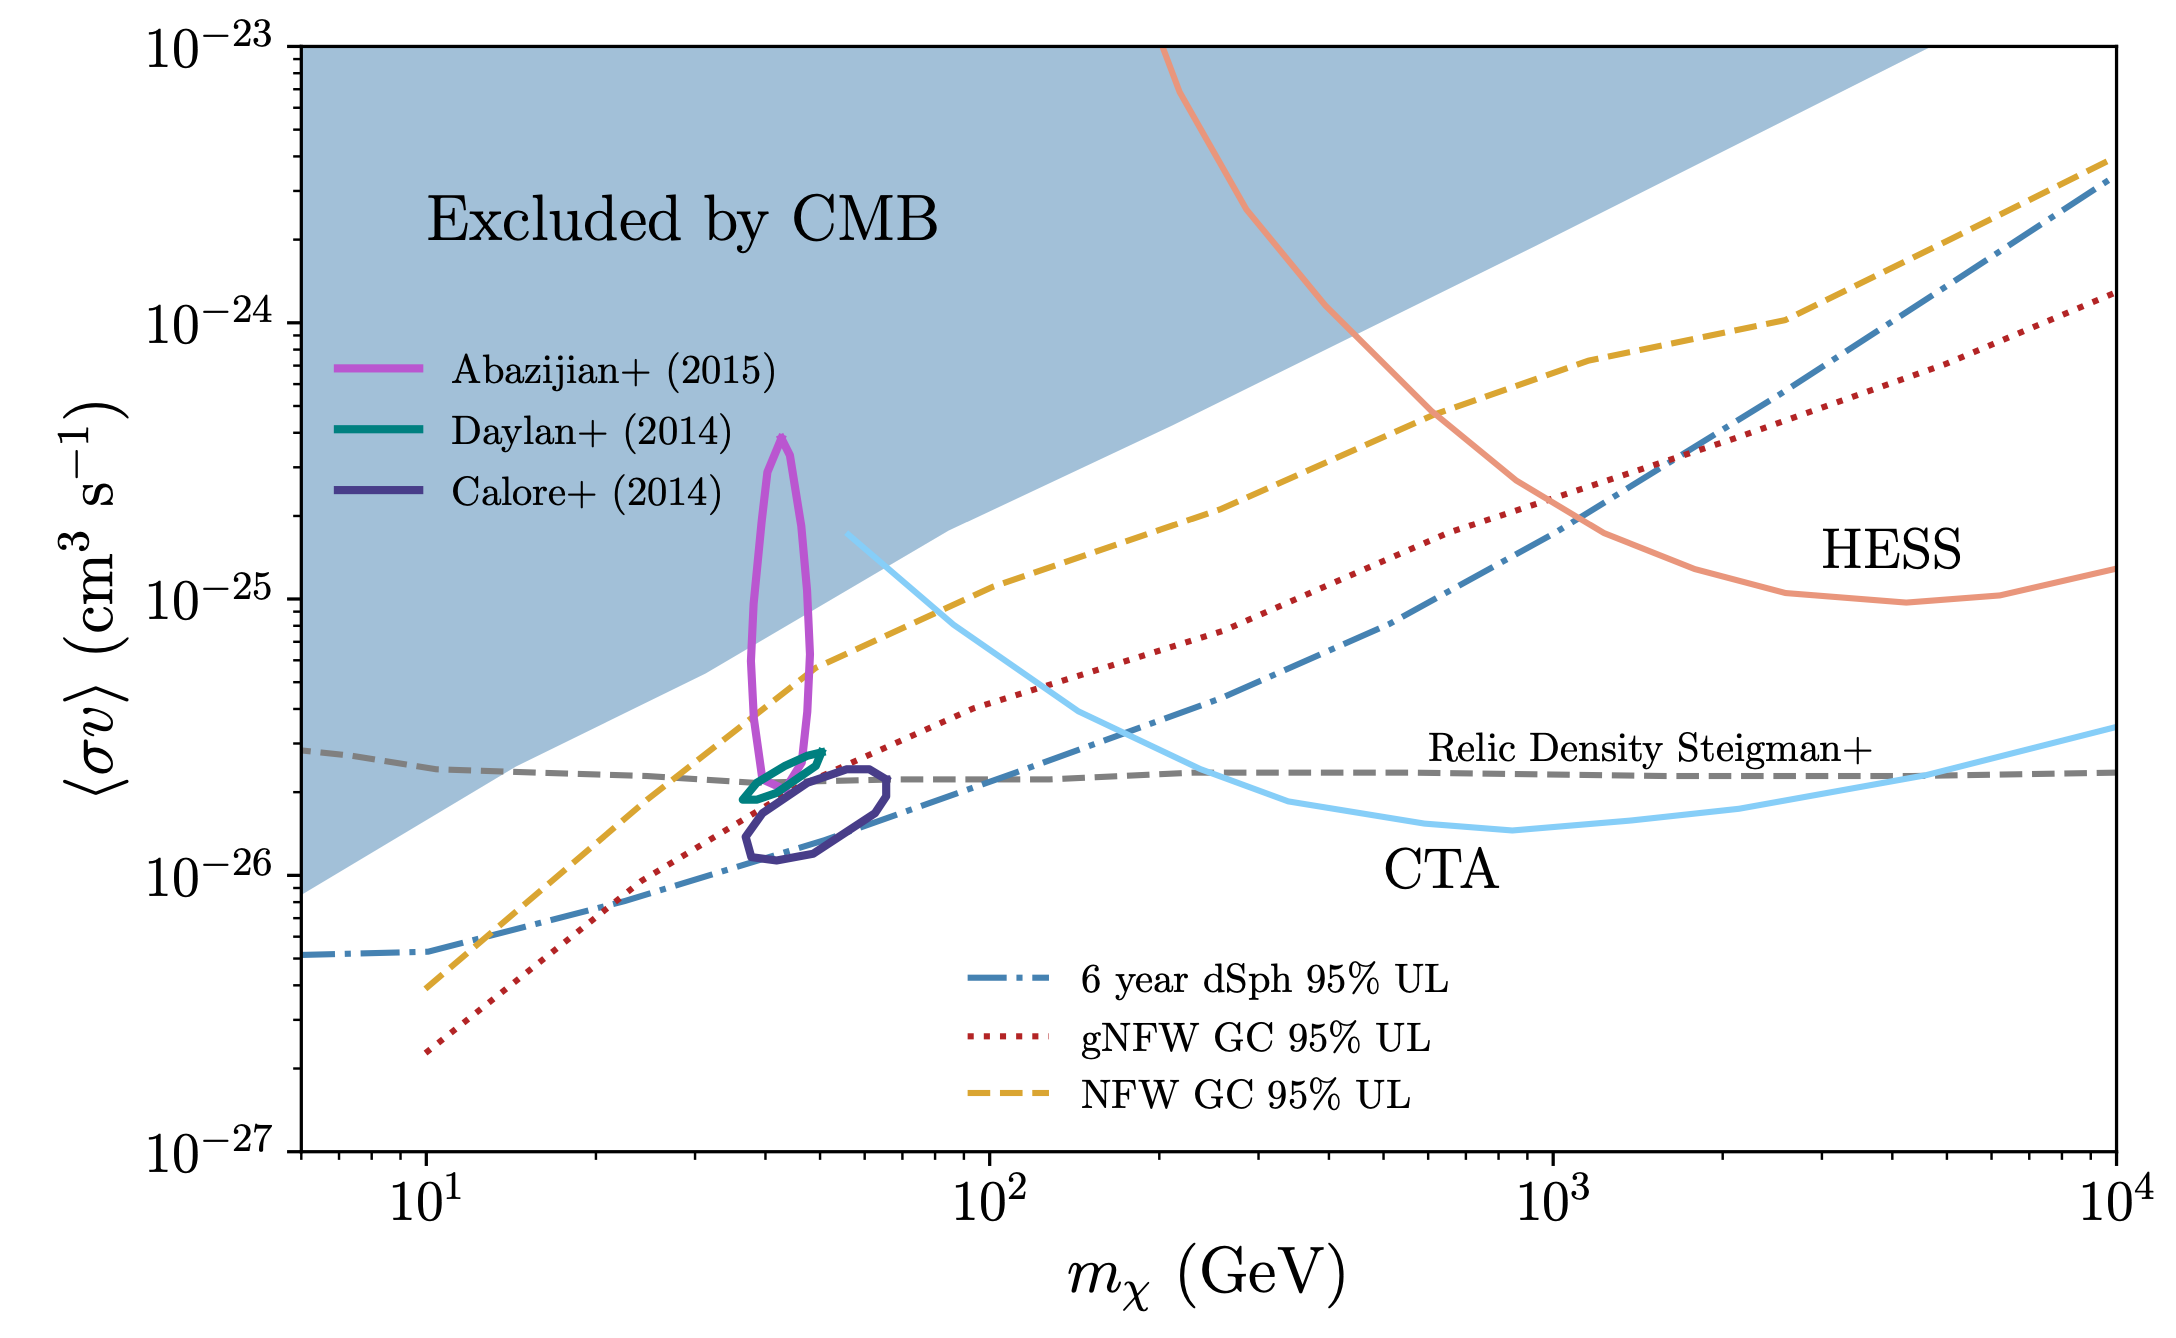
\includegraphics[width=0.95\textwidth]{figures/darkmatter/pdg_indirectdetection2020.png}
    \caption{Constraints placed on the self-annihilation cross-section for WIMPs with mass \(m_{\chi}\) by indirect detection experiments. Figure reproduced from Ref.~\cite{Tanabashi2018}.}
    \label{fig:dm:searches:id:overview}
\end{figure}

\subsection{Searches for dark matter at particle colliders}
\label{sec:dm:searches:collider}
Hadron collider searches (c.f. Ref.~\cite{Buchmueller2017} for a review) aim to detect signals of WIMPs produced when colliding proton beams in a controlled laboratory environment. Dark matter particles leave no trace in the detectors surrounding the collision point due to their feeble interactions with SM particles. The absence of a reconstructed particle trajectory allows inferring the presence of dark matter using momentum conservation in the plane perpendicular to the colliding beams. As the net transverse momentum before the collision is zero, it must also be so after the collision. An imbalance in the transverse plane is quantified by the missing transverse momentum \met, which is obtained as the negative vector sum of the transverse momenta of all detected particles. The characteristic signature for WIMP production at particle colliders is the observation of significant \met in association with one or more additional SM particles. This signature is known as ``\(\met + X\)'' and underpins the searches presented in this dissertation. The interaction between SM and dark matter particles typically takes place via a spin-1 or spin-0 mediator. The ATLAS and CMS experiments carry out a range of \(\met + X\) searches:
\begin{itemize}
    \item \met + jets,
    \item \met + photon \Pgg or weak vector boson \PWpm / \PZ,
    \item \met + heavy flavour quarks.
    \item \met + SM Higgs boson \Ph,
\end{itemize}
The \met + jets search~\cite{EXOT-2016-27,CMS-EXO-16-048} is one of the most inclusive types of searches by considering final states with one or more jets originating from initial state radiation. The accurate theoretical description of SM background processes, which is improved by data-driven methods, establishes the sensitivity to potential signals in the tails of the \met distribution.
Similarly, dark matter particles may be produced in association with a vector boson radiated off from a quark in the initial state.
The \met + photon searches~\cite{EXOT-2016-32,CMS-EXO-16-039} benefit from a very clean signature of \met and a high-energetic photon. The much lower backgrounds compared to the \met + jets search make up for the smaller production cross-section than for QCD radiation. The \met + weak vector boson searches can investigate different decay modes of the vector boson. While a leptonically decaying \PZ boson~\cite{HIGG-2016-28} also presents a very clean signature, the hadronic decay channel~\cite{CMS-EXO-16-037} is appealing due to the larger branching fraction.
The searches targeting \met + heavy flavour quarks~\cite{SUSY-2016-18,CMS-EXO-18-010,CMS-EXO-16-051,CMS-EXO-16-049} can probe dark matter production via the exchange of spin-0 mediators.
Finally, searches targeting the \met + SM Higgs boson final state can investigate the various decay modes of the Higgs boson~\cite{CMS-EXO-18-011}. The decay to \bquarks~\cite{EXOT-2016-25,ATLAS-CONF-2018-039} if favoured by having the largest branching fraction. Searches also explore the cleaner \HepProcess{\Ph \to \Pgtpm \Pgtmp}~\cite{CMS-EXO-16-055} and \HepProcess{\Ph \to \Pgg \Pgg}~\cite{HIGG-2016-18} final states with smaller branching fractions. Searches probing the invisible decay of the Higgs boson in vector-boson-fusion topology or associated production with vector bosons~\cite{HIGG-2016-28} serve as another test of the WIMP hypothesis.
To date, no collider search has made claims of discovery of dark matter.

A second approach in constraining dark matter models at colliders is searching for the visible decays of the mediators. Assuming the existence of such a mediator, at least the visible mediator decay to the same SM particles which produced the mediator -- quarks or gluons --- is guaranteed. Also, possible decays to leptons are considered. The signature of visible mediator decays is a narrow excess in the otherwise smoothly falling background spectrum of the invariant mass of two jets or leptons with the largest momentum. The ATLAS and CMS experiments carry out a range of dijet~\cite{EXOT-2019-03,CMS-EXO-16-032} or dilepton searches~\cite{CMS-EXO-16-056,}. While the high-mass dijet resonance searches constrain the mediator mass from \SI{1.5}{\tera\electronvolt} to \SI{3.5}{\tera\electronvolt}, the searches for low-mass dijet resonances are limited by the process high rates. Searches in this regime are enabled by recording only a limited amount of information of the full event record~\cite{EXOT-2016-20} or by requiring the presence of a resonance produced in association with an additional high-energetic particle or jet~\cite{EXOT-2018-05}.

The current status and perspectives for collider based dark matter searches are presented in \Cref{sec:outlook}.


\section{Theoretical frameworks for dark matter production at particle colliders}
\label{sec:dm:models}
The theoretical frameworks predicting the production of WIMPs are an indispensable part of collider searches. They guide the design and optimisation of the searches by elucidating the phenomenology of potential dark matter particle candidates in specific final states. In addition, they allow connecting the results of collider searches with direct and indirect detection experiments.

The range of models predicting dark matter production at the LHC varies in generality and plausibility. The two end-points of the spectrum are defined by the effective field theory (EFT) approach and complete theories, such as supersymmetry. \Cref{fig:dm:models:overview} shows an overview of theoretical frameworks describing dark matter production at particle colliders with varying degrees of completeness and complexity.
\begin{figure}[htbp]
    \centering
    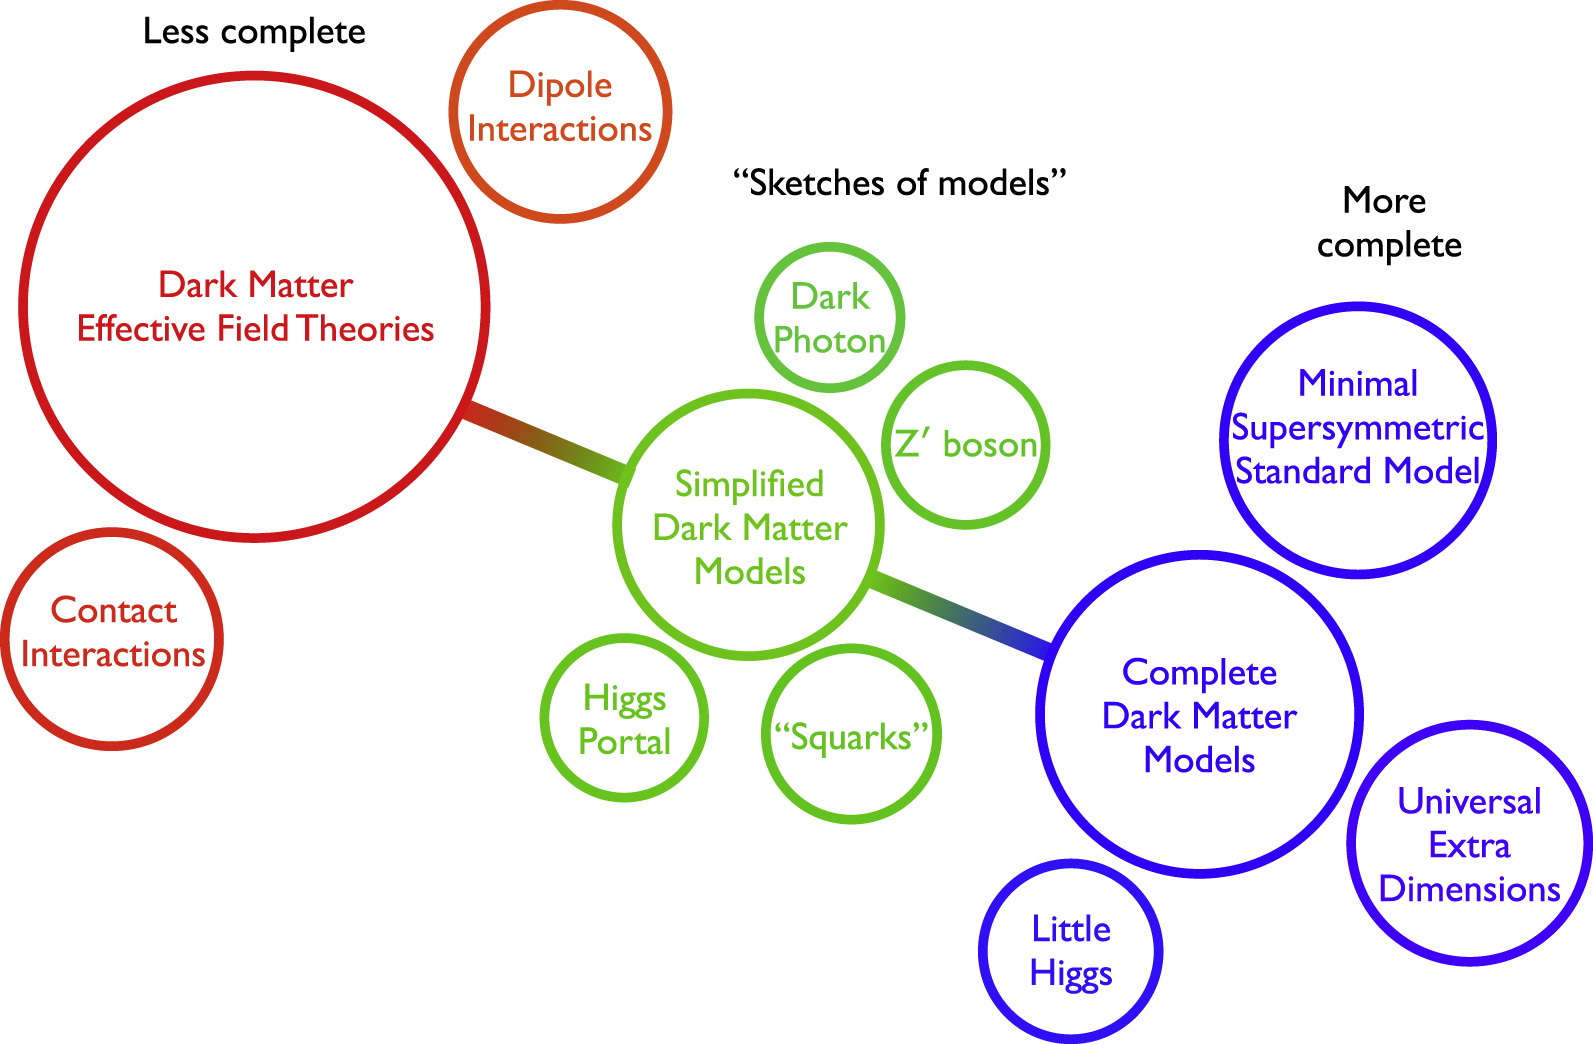
\includegraphics[width=0.95\textwidth]{figures/darkmatter/models.jpg}
    \caption{Overview of theoretical frameworks describing dark matter production at particle colliders. The models range from dark matter effective field theory, over various simplified models, to complete dark matter models. Figure reproduced from Ref.~\cite{Abdallah2015}.}
    \label{fig:dm:models:overview}
\end{figure}

The effective field theory (EFT) approach introduces the WIMP as the only additional state which is accessible at the LHC and describes its interaction with SM particles through a four-point effective contact interaction. Similar to Fermi's theory of weak interactions, heavy intermediate states are mapped to effective operators, which are characterised by the energy scale of the interaction.
Complete theoretical frameworks, on the other hand, are well-motivated and consistent theories with perturbative ultraviolet (UV) completions. They make specific predictions for invisible, heavy particles with mass at the electroweak scale. Typically, these complete theories are characterised by a large number of model parameters.

While the LHC experiments also have a broad array of searches in the context of complete theories, the dedicated LHC dark matter searches follow a theory-agnostic approach by specifying only the interaction between SM particles and WIMPs relevant to the signature of dark matter pair production.

It has been shown that the EFT approach is overly simplistic to capture the phenomenology of more complete models fully. Their kinematic distributions differ significantly from the ones obtained in an EFT description. Moreover, the EFT approach breaks down at the \si{\tera\electronvolt} energy scale probed in LHC interactions, as the momentum transfer in the process is sufficient to resolve the underlying processes.
As a consequence, the preferred theoretical framework of LHC dark matter searches are \emph{simplified models}, which make explicit assumptions about at least two additional states: a WIMP and a particle mediating the interaction between WIMP and SM particles. Scenarios with an SM mediator are almost ruled out, therefore suggesting the mediator to be a yet-undiscovered particle. Although simplified models are characterised by only a small number of parameters and make no assumptions about extended particle sectors, they can be designed to be fully consistent at all energy scales.

The searches for dark matter presented in this dissertation are motivated by a range of simplified models with varying degree of complexity. The following paragraphs discuss a simplified model for dark matter production with a spin-1 \PZprime mediator, two simplified models with an extended Higgs sector, and a simplified model with two mediators.

\subsection{Simplified model for dark matter production with a spin-1 \PZprime mediator}
\label{sec:dm:models:dmsimp}
The simplified model with a vector or axial-vector mediator (\(V/A\) simplified model)~\cite{Abercrombie2019} is a minimal extension of the SM describing the production of dark matter particles via \(s\)-channel exchange. The model postulates a Dirac fermion dark matter particle \(\chi\) with mass \mchi, which is charged under an additional \(\text{U}(1)\) gauge symmetry. Assuming that also some SM particles are charged under this group, dark matter pair production can occur via the exchange of a new \PZprime gauge boson of mass \mZp, which is referred to as the \emph{mediator}. Both vector and axial-vector couplings between the spin-1 mediator are possible. The corresponding interaction Lagrangian densities are (neglecting mediator couplings to leptons with coupling strength \gl)
\begin{align}
    \mathcal{L}_{\text{vector}} &= \gq \sum_{q=\Pup, \Pdown, \Pstrange, \Pcharm, \Pbottom, \Ptop} \PZprime_{\mu} \overline{q} \gamma^{\mu} q + \gchi \PZprime_{\mu} \overline{\chi} \gamma^{\mu} \chi \\
    \mathcal{L}_{\text{axial-vector}} &= \gq \sum_{q=\Pup, \Pdown, \Pstrange, \Pcharm, \Pbottom, \Ptop} \PZprime_{\mu} \overline{q} \gamma^{\mu} \gamma^{5} q + \gchi \PZprime_{\mu} \overline{\chi} \gamma^{\mu} \gamma^{5} \chi
    \label{eq:dm:model:dmsimp}
\end{align}

The mediator couples universally to all quarks and leptons with the coupling strengths \gq and \gl, respectively, and couples to dark matter particles \(\chi\) with coupling strength \gchi~\cite{Albert2019}. The universal coupling to all quarks or leptons ensures that the general structure of flavour-changing neutral current processes is preserved in the extension of the SM via Minimal Flavour Violation~\cite{DAmbrosio2002}. Assuming that no additional visible or invisible decays contribute to the width of the mediator and ignoring possible decays to leptons, the minimal width is fixed by the couplings \gq and \gchi. The minimal widths for the vector and axial vector mediator are
\begin{align}
    \Gamma^{V}_{\text{min}} = & \Gamma^{V}_{\HepProcess{\chi \chi}} + \Gamma^{V}_{\HepProcess{\Pq\Pq}}\\
   = & \frac{\gchi^2 \mZp}{12 \pi} \left(1 + \frac{2 \mchi^2}{\mZp^2}\right) \beta_{\chi} \theta(\mZp - 2 \mchi) \nonumber \\
    & + \sum_{q=\Pup, \Pdown, \Pstrange, \Pcharm, \Pbottom, \Ptop} \frac{3 \gq^2 \mZp}{12 \pi} \left(1 + \frac{2 m_{\Pq}^2}{\mZp^2}\right) \beta_{\Pq} \theta(\mZp - 2 m_{\Pq}) \nonumber \\
	\Gamma^{A}_{\text{min}} = & \Gamma^{A}_{\HepProcess{\chi \chi}} + \Gamma^{A}_{\HepProcess{\Pq\Pq}}\\
   = & \frac{\gchi^2 \mZp }{12 \pi} \beta^3_{\chi} \theta(\mZp - 2 \mchi) \nonumber \\
	& + \sum_{q=\Pup, \Pdown, \Pstrange, \Pcharm, \Pbottom, \Ptop} \frac{3 \gq^2 \mZp}{12 \pi} \beta^3_{\Pq} \theta(\mZp - 2 \mchi), \nonumber
\end{align}
where \(\theta\) denotes the Heaviside step function and \(\beta_f = \sqrt{1 - 4 m_{f}^2 / \mZp^2}\) is the velocity of the fermion \(f\) with mass \(m_{f}\) in the rest frame of the \PZprime mediator.

Under the minimal width assumption, the model is specified by the set of parameters shown in \Cref{tab:dm:models:dmsimp:parameters}.
\begin{table}[hbt]
\caption{Parameters in the \(V/A\) simplified model}
\label{tab:dm:models:dmsimp:parameters}
\centering
\begin{tabular}{ll}
\toprule
Parameter & Description \\
\midrule
\mZp & \PZprime mediator mass \\
\mchi & dark matter particle mass \\
\gq & coupling strength of \PZprime mediator to quarks \\
\gl & coupling strength of \PZprime mediator to leptons \\
\gchi & coupling strength of \PZprime mediator to dark matter particles \\
\bottomrule
\end{tabular}
\end{table}

Both the vector mediator and the axial-vector mediator model are available in event generators up to next-to-leading order (\NLO) accuracy in QCD.

\subsection{Simplified model with an extended Higgs sector and a pseudo-scalar mediator}
\label{sec:dm:models:ahdm}
The \ahdm~\cite{Bauer2017} is a self-consistent simplified model with an extended Higgs sector, allowing the model to be embedded in a UV-complete and renormalisable framework. It is based on a Two-Higgs-doublet model (2HDM)~\cite{Branco2012} with five physical scalar states in the Higgs sector and an additional pseudo-scalar mediator.

The 2HDM potential for the two Higgs doublets \(H_{1}, H_{2}\) is given by
\begin{align}
    V_{H} = &\mu_{1} H_{1}^{\dagger} H_{1} + \mu_{2} H_{2}^{\dagger} H_{2} + (\mu_{3} H_{1}^{\dagger} H_{2} + \text{h.c.}) \nonumber \\
    & + \lambda_{1} (H_{1}^{\dagger} H_{1})^2 + \lambda_{2} (H_{2}^{\dagger} H_{2})^2 + \lambda_{3} (H_{1}^{\dagger} H_{1}) (H_{2}^{\dagger} H_{2}) \nonumber \\
    & + \lambda_{4} (H_{1}^{\dagger} H_{2}) (H_{2}^{\dagger} H_{1}) + \left[\lambda_{5} (H_{1}^{\dagger} H_{2})^2 + \text{h.c.}\right],
\end{align}
where \(\text{h.c.}\) denotes the Hermitian conjugate and \(\mu_{i}, i=1,2,3\) and \(\lambda_{i}, i=1,\dots,5\) are free parameters. The potential is CP-conserving and has a softly broken \(\mathbb{Z}_{2}\) custodial symmetry to suppress flavour-changing neutral currents. The Higgs doublets have the vacuum expectation values \(\langle H_{i} \rangle = (0, v_{i} / \sqrt{2})^{T}, i=1,2\) with \(v = \sqrt{v_{1}^2 + v_{2}^2} = \SI{246}{\giga\electronvolt}\) and their ratio defines \(\tan \beta = v_2 / v_1\). The physical CP-even states \Ph and \PH result from mixing of the  neutral CP-even weak eigenstates with a corresponding mixing angle \(\alpha\). The extended Higgs sector contains also two charged states \PHpm of identical mass.

The interaction term for the pseudo-scalar mediator \(P\)
\begin{align}
    V_{P} = \frac{1}{2} m_{P}^2 P^2 + P(i b_{P} H_{1}^{\dagger} H_{2} + \text{h.c.}) + P^2 (\lambda_{P_{1}} H_{1}^{\dagger} H_{1} + \lambda_{P_{2}} H_{2}^{\dagger} H_{2}),
\end{align}
with the pseudo-scalar mass parameter \(m_{P}\) and the portal couplings \(b_{P}, \lambda_{P_{1}}, \lambda_{P_{2}}\),
mixes the mediator with the CP-odd state in the extended Higgs sector with mixing angle \(\theta\). The resulting physical CP-odd states are \(a\) and \PA.

The dark matter particle \(\chi\) is a Dirac fermion with mass \(m_{\chi}\). The pseudo-scalar mediator couples to the dark matter particle with the real Yukawa coupling \(y_{\chi}\) via
\begin{align}
    \mathcal{L}_{\chi} = - i y_{\chi} P \overline{\chi} \gamma_{5} \chi.
\end{align}

The alignment limit \(\sin{(\beta - \alpha)} = 1\) is assumed, allowing the identification of the lightest CP-even scalar \Ph with the SM Higgs boson. A type-II 2HDM coupling structure is assumed, letting up- and down-type quarks couple to separate doublets. The model is specified by the set of 14 parameters shown in \Cref{tab:dm:models:ahdm:parameters}.
\begin{table}[hbt]
\caption{Parameters in the \ahdm simplified model}
\label{tab:dm:models:ahdm:parameters}
\centering
\begin{tabular}{ll}
\toprule
Parameter & Description \\
\midrule
\(\alpha\) & mixing angle of neutral CP-even weak eigenstates \\
\(\tan{\beta}\) & ratio of Higgs doublet vacuum expectation values \\
\(\theta\) & mixing angle of neutral CP-odd weak eigenstates \\
\(v\) & electroweak vacuum expectation value \\
\(\lambda_{3}, \lambda_{P_{1}}, \lambda_{P_{2}}\) & quartic couplings of scalar bosons \\
\(m_{\Ph}, m_{\PH}\) & masses of neutral CP-even Higgs bosons \\
\(m_{a}, m_{\PA}\) & masses of neutral CP-odd Higgs bosons \\
\(m_{\PHpm}\) & charged Higgs bosons mass \\
\(m_{\chi}\) & dark matter particle mass \\
\(y_{\chi}\) & Yukawa coupling of dark matter particle \\
\bottomrule
\end{tabular}
\end{table}

The \ahdm model is characterised by a rich phenomenology so that it can be probed by all \met + X searches, which are discussed in \Cref{sec:dm:searches:collider}. In particular, the \met + Higgs boson and \met + \PZ boson final states are expected to provide leading constraints in the theoretically best-motivated region of the parameter space.

\subsection{\zhdm simplified model}
\label{sec:dm:models:zp2hdm}
The \zhdm~\cite{Berlin2014} is another simplified model with an extended Higgs sector. It is based on a 2HDM (c.f. the discussion in \Cref{sec:dm:models:ahdm}) with an additional \(\text{U}(1)_{\PZprime}\) symmetry, which gives rise to a \PZprime boson. The \PZprime boson can mix with the \PZ boson. It is implicitly assumed that there is a mechanism for generating the \PZprime boson mass in a gauge-invariant way.

After symmetry breaking, the two Higgs doublets can be parametrised as
\begin{align}
H_{1} &= \begin{pmatrix} -\PHpm \sin \beta \\ v_{1} - \Ph \sin \alpha + \PH \cos \alpha - i \PA \sin \beta \end{pmatrix}\\
H_{2} &= \begin{pmatrix} \PHpm \cos \beta \\ v_{2} + \Ph \cos \alpha + \PH \sin \alpha + i \PA \cos \beta \end{pmatrix},
\end{align}
where similar conventions for denoting the Higgs doublets, the states in the extended Higgs sector and the mixing angles have been adopted as in \Cref{sec:dm:models:ahdm}.
The alignment limit \(\sin{(\beta - \alpha)} = 1\) is assumed, allowing the identification of the lightest CP-even scalar \Ph with the SM Higgs boson. The model specifies a type-II 2HDM coupling structure, letting up- and down-type quarks couple to separate doublets.
As only the right-handed up-type quarks \(\Pqu_{i, R}\) and the Higgs doublet \(H_{1}\) are charged under \(\text{U}(1)_{\PZprime}\), the \PZprime boson only couples to the Higgs doublet which couples to the up-type quarks and to right-handed quarks.
The CP-odd physical state \PA in the extended Higgs sector couples to dark matter particles.

The model is specified by the set of nine parameters shown in \Cref{tab:dm:models:zhdm:parameters}.
\begin{table}[hbt]
\caption{Parameters in the \zhdm simplified model}
\label{tab:dm:models:zhdm:parameters}
\centering
\begin{tabular}{ll}
\toprule
Parameter & Description \\
\midrule
\(\alpha\) & mixing angle of neutral CP-even weak eigenstates \\
\(\tan{\beta}\) & ratio of Higgs doublet vacuum expectation values \\
\(m_{\Ph}, m_{\PH}\) & masses of neutral CP-even Higgs bosons \\
\(m_{\PHpm}\) & mass of charged Higgs bosons \\
\mA & neutral CP-odd Higgs boson mass \\
\mZp & \PZprime boson mass \\
\(g_{\PZprime}\) & coupling strength of the \PZprime boson \\
\mchi & dark matter particle mass\\
\bottomrule
\end{tabular}
\end{table}

The model describes resonant production of a \PZprime boson, which subsequently decays into the SM Higgs boson \Ph and the CP-odd Higgs boson \PA. The latter enables dark matter pair production due to its large branching fraction to dark matter.

\subsection{Two mediator dark matter model}
\label{sec:dm:models:2mdm}
The two mediator dark matter model~\cite{Duerr2016,Duerr2017} (2MDM model) is a consistent simplified model with a \PZprime boson and a dark Higgs boson as mediators. The model postulates a Majorana fermion as dark matter particle \(\chi\), a complex Higgs field \(S\) and an additional \(\text{U}(1)_{\PZprime}\) gauge group. It satisfies the requirements of gauge invariance and perturbative unitarity by incorporating more features of complete theories: the masses of the fermionic dark matter particle and of the \PZprime boson are generated by spontaneous symmetry breaking of the \(\text{U}(1)_{\PZprime}\) group. The symmetry breaking gives rise to the dark Higgs boson \(s\). The dark matter particle \(\chi\) with mass \(m_{\chi}\) couples via axial coupling to the \PZprime boson. The interaction Lagrangian density is
\begin{align}
    \mathcal{L}_{\chi} = - \frac{1}{2} g_{\chi} \PZprime^{\mu} \overline{\chi} \gamma^{5} \gamma_{\mu} \chi - g_{\chi} \frac{m_{\chi}}{m_{\PZprime}} s \overline{\chi} \chi + 2 g_{\chi} \PZprime^{\mu} \PZprime_{\mu} (g_{\chi} s^2 + m_{\PZprime} s).
\end{align}
with the four independent parameters
\begin{itemize}
	\item dark matter particle mass \mchi,
	\item \PZprime boson mass \mZp,
	\item dark Higgs boson mass \ms,
	\item \(\gchi = g_{\PZprime} q_{\chi}\) dark matter coupling, with the \(\text{U}(1)_{\PZprime}\) gauge coupling \(g_{\PZprime}\) and charge of the dark matter particle \(q_{\chi} = q_{S} / 2\).
\end{itemize}

The dark sector is coupled to the SM by postulating vector couplings of the \PZprime to quarks (\Pq) by gauging baryon number. The corresponding interaction Lagrangian is
\begin{align}
    \mathcal{L}_{q} = - \gq \PZprime^{\mu} \Paq \gamma_{\mu} \Pq
\end{align}
with the coupling strength of the \PZprime boson to quarks \gq. Axial-vector couplings and couplings to leptons are neglected for simplicity.


The model is specified by the set of five parameters shown in \Cref{tab:dm:models:2mdm:parameters}.
\begin{table}[hbt]
\caption{Parameters in the two mediator dark matter simplified model}
\label{tab:dm:models:2mdm:parameters}
\centering
\begin{tabular}{ll}
\toprule
Parameter & Description \\
\midrule
\mchi & dark matter particle mass \\
\mZp & \PZprime mediator mass \\
\ms & the dark Higgs boson mass \\
\gchi & coupling strength of \PZprime mediator to dark sector \\
\gq & coupling strength of \PZprime mediator to quarks \\
\(\theta\) & mixing angle between the SM Higgs boson \\
           & and the dark Higgs boson \\
\bottomrule
\end{tabular}
\end{table}

The model can be thought of as a combination of two simplified models: one with a spin-1 mediator (c.f. \Cref{sec:dm:models:dmsimp}) and one with a spin-0 mediator. In this dissertation, the resonant production of a dark Higgs boson decaying to SM particles is investigated.

Non-zero mixing between the dark Higgs boson and the SM Higgs boson with mixing angle \(\theta\) ensures that the dark Higgs boson is unstable and can instantly decay into SM states. Consequentially, the dark Higgs boson inherits the branching fractions of an SM-like Higgs boson with mass \ms, which are shown in \Cref{fig:dm:models:2mdm:darkhiggsbranching}.

\begin{figure}[htbp]
    \centering
    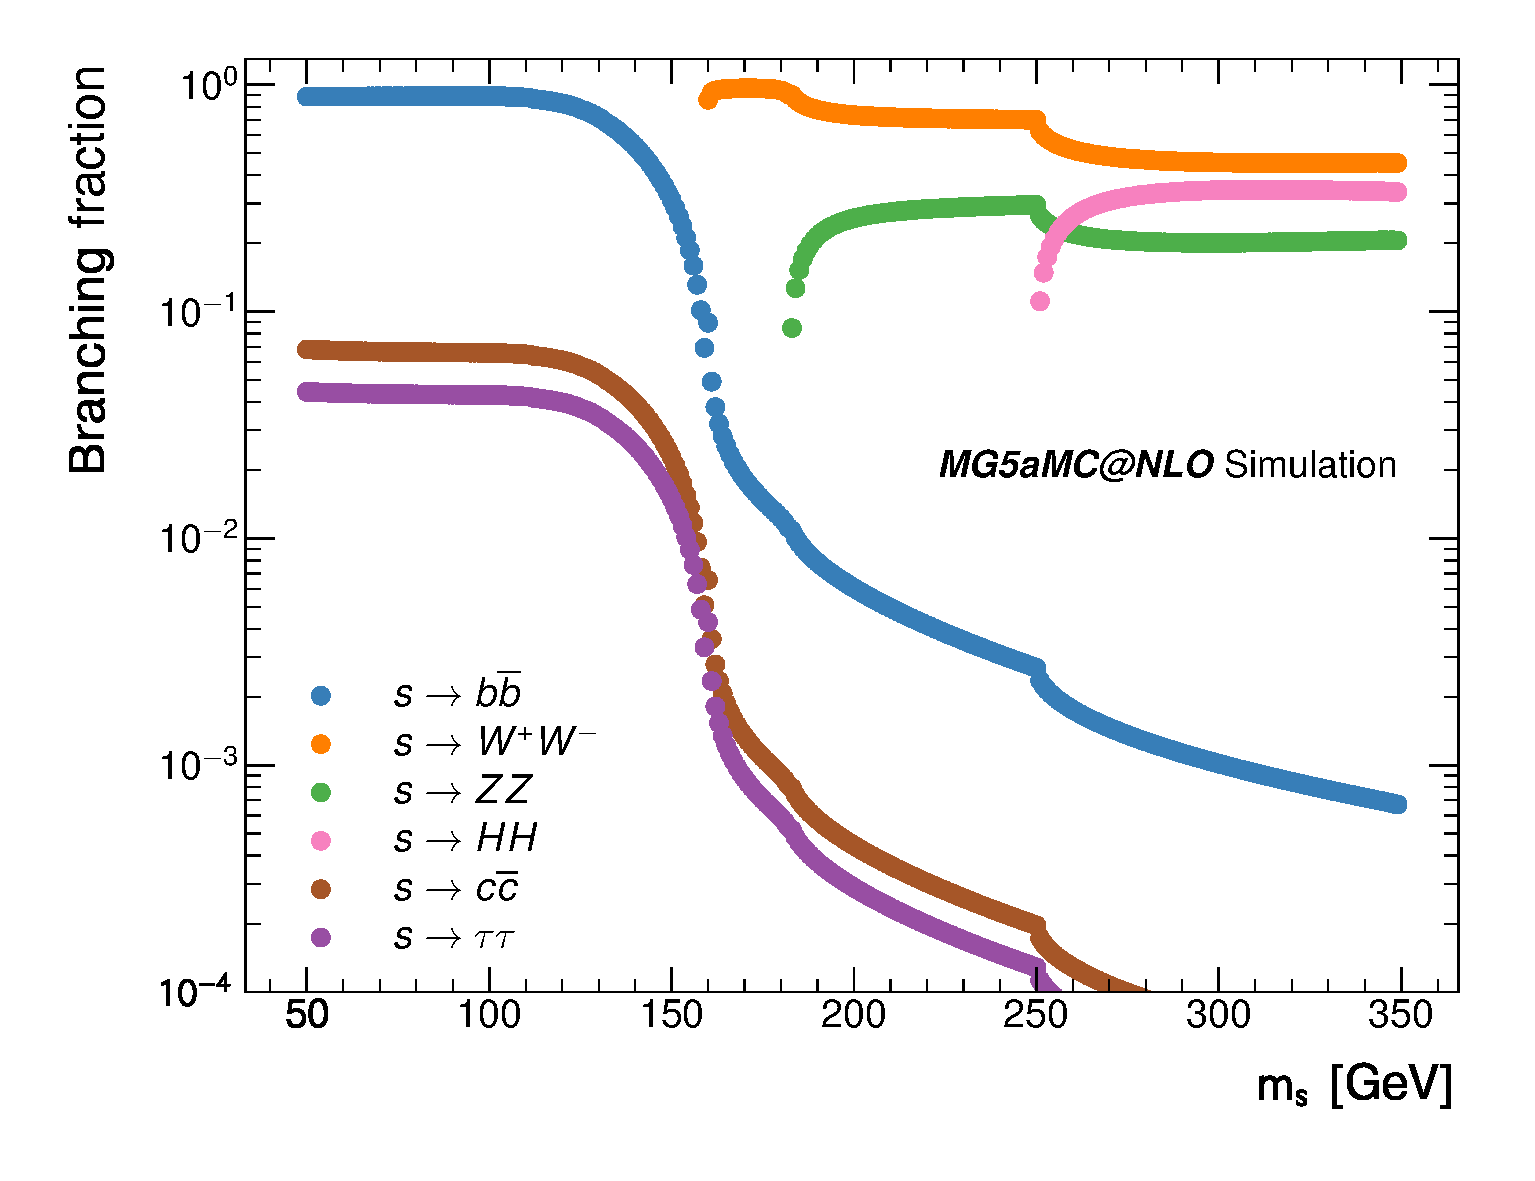
\includegraphics[width=0.95\textwidth]{figures/darkmatter/darkhiggs_branchingfraction.pdf}
    \caption{Branching fractions of dark Higgs boson decays to SM particles (produced on-shell) in dependence of \ms.}
    \label{fig:dm:models:2mdm:darkhiggsbranching}
\end{figure}
